
\chapter{Opetopes}
\lbl{ch:opetopic}

\chapterquote{%
John Dee [\ldots] summoned angels of dubious celestial provenance by
invoking names like Zizop, Zchis, Esiasch, Od and Iaod}{%
Eco~\cite{Eco}}


\noindent
Operads lead inescapably into geometry.  In this chapter we see that as
soon as the notion of generalized operad is formulated, the notion of
opetope is unavoidable.  Opetopes are something like simplices: they are a
completely canonical family of polytopes, as pervasive in
higher-dimensional algebra as simplices are in geometry.

In~\ref{sec:opetopes} opetopes are defined and their geometric
representation explained.  Intertwined with the definition of opetope is
the definition of a certain sequence $(T_n)_{n\in\nat}$ of cartesian
monads; we also look at $T_n$-multicategories and their relation to
symmetric multicategories.  Section~\ref{sec:pds} is formally about
$T_n$-structured categories (in the sense of~\ref{sec:struc}); translated
into geometry, this means diagrams of opetopes pasted together.

As we shall see, there is a category of $n$-dimensional pasting diagrams
for each natural number $n$.  When $n=1$ this is the category $\scat{D}$%
%
\index{augmented simplex category $\scat{D}$}
%
of
finite totally ordered sets (the augmented simplex category); when $n=2$ it
is a category of trees, as found in parts of quantum algebra.
In~\ref{sec:trees} we analyse the category of trees in some detail.  Some
of this is analogous to some of the standard analysis of $\scat{D}$: see
for instance Mac Lane~\cite[VII.5]{MacCWM}, where the monics, epics,
primitive face and degeneracy maps, and standard factorization properties
are all worked out, and the universal role of $\scat{D}$ (as the free
monoidal category containing a monoid) is established.

Opetopes were invented by Baez%
%
\index{Baez, John}
%
and Dolan~\cite{BDHDA3}%
%
\index{Dolan, James}
%
so that they could
frame a definition of weak $n$-category.  The strategy is simple: opetopes
together with face maps form a category, a presheaf on that category is
called an opetopic set, and a weak $n$-category is an opetopic set with
certain properties.  This is like both the definition of Kan complex (a
simplicial set with horn-filling properties) and the definition of
representable multicategory (a multicategory with universality
properties,~\ref{defn:repn-multi}).  Opetopic sets are discussed
in~\ref{sec:ope-sets}, and opetopic definitions of weak $n$-category
in~\ref{sec:ope-n}.

We finish~(\ref{sec:many}) with a short section on the `many%
%
\index{many in, many out}
%
in, many out'
approach to higher-dimensional category theory.  Opetopes arise from the
concept of operations with many inputs and a single output.  We could start
instead with the concept of operations having both many inputs and many
outputs, and try to construct shapes analogous to opetopes.  But this turns
out to be impossible, as we see.  (Formally, 3-computads do not form a
presheaf category.)  This does not mean that it is hopeless to try to
develop a many-in, many-out framework for higher categorical structures,
but it does mean that such a framework would be qualitatively different
from the simplicial, cubical, globular, and opetopic frameworks, in each of
which there is a genuine category of shapes.





\section{Opetopes}
\lbl{sec:opetopes}


The following table shows some of the types of generalized operad that we
have met.  As usual, $T$ is a cartesian monad on a cartesian category
$\Eee$.
%
\begin{center}
\begin{tabular}{lll}
$\Eee$		&$T$			&$T$-operads			\\
		&			&				\\
$\Set$		&identity		&monoids			\\
$\Set$		&free monoid		&plain operads		\\
$\Set^\nat \eqv \Set/\nat$	&
		 free plain operad	&
			(see~\ref{eg:mti-free-cl-opd})
\end{tabular}
\end{center}
%
Each row is generated automatically from the last by taking $T$ to be
`free%
%
\index{generalized operad!free}
%
operad of the type in the last row'.  Technicalities aside, it is clear
that this table can be continued indefinitely.

This gives an absolutely fundamental infinite sequence of categories
$\Eee$, monads $T$, and types of generalized operad.  The bulk of this
chapter consists of working out what they look like.  It is plain
from the first few rows that there will be some geometrical content---for
instance, in the third row, the operations in a $T$-operad are indexed by
trees (Example~\ref{eg:mti-free-cl-opd}).

The table can be compared with that of Ginzburg%
%
\index{Ginzburg, Victor}
%
and
Kapranov~\cite[p.~204]{GiKa}.%
%
\index{Kapranov, Mikhail}
%
 They include columns marked `Geometry'
(whose entries are `vector bundles', `manifolds', and `?(moduli spaces)'),
`Linear Physics', and `Nonlinear Physics'.  Their table, like the one
above, has only three rows.  Here we show how to continue forever---in our
columns, at least.

To do this formally we need to recall the results on free operads
in~\ref{sec:free-mti}.  There we met the concept of `suitable' categories
and monads and saw that they provided a good context for free operads.
Specifically, let $T$ be a suitable monad on a suitable category $\Eee$
with a terminal object.  Then Theorem~\ref{thm:free-fixed} tells us that
the forgetful functor
\[
\Cartpr\hyph\Operad \go \Eee/T1
\]
sending a $T$-operad to its underlying $T$-graph has a left adjoint, that
the induced monad (`free $T$-operad') on $\Eee/T1$ is suitable, and that
the category $\Eee/T1$ is suitable.  Trivially, $\Eee/T1$ has a terminal
object.  Also, Theorem~\ref{thm:free-gen} tells us that the category of
sets and the identity monad on it are both suitable.  This makes possible:
%
\begin{defn}	\lbl{defn:opetopic-monads}
For each $n\in\nat$, the suitable category $\Eee_n$%
% 
\glo{nthopecat}
% 
and the suitable
monad $T_n$%
% 
\glo{nthopemonad}%
%
\index{opetopic!monad}
% 
on $\Eee_n$ are defined inductively by
%
\begin{itemize}
\item $\Eee_0 = \Set$ and $T_0 = \id$
\item $\Eee_{n+1} = \Eee_n / T_n 1$ and
$T_{n+1} = (\textrm{free } T_n \textrm{-operad}).$ 
\end{itemize}
\end{defn}

In fact, there is for each $n\in\nat$ a set $O_n$%
% 
\glo{nopes}
% 
such that $\Eee_n$ is
canonically isomorphic to $\Set/O_n$.  (Recall also from
p.~\pageref{eq:Set-slice-power} that $\Set/O_n \eqv \Set^{O_n}$.)  First,
$O_0 = 1$.  Now suppose, inductively, that $n\geq 0$ and $\Eee_n \iso
\Set/O_n$.  The terminal object of $\Set/O_n$ is $(O_n \goby{1} O_n)$, so
if we put
\[
\bktdvslob{O_{n+1}}{t}{O_n} = T_n \bktdvslob{O_n}{1}{O_n}
\]
then we have
\[
\Eee_{n+1} = 
\frac{\Eee_n}{T_n 1} \iso
\frac{\Set/O_n}{O_{n+1} \goby{t} O_n} \iso
\frac{\Set}{O_{n+1}}.%
% 
\glo{opetgt}
% 
\]
This gives an infinite sequence of sets and functions
\[
\cdots 
\ 
\goby{t} 
O_{n+1} 
\goby{t} 
O_n 
\goby{t} 
\ 
\cdots
\ 
\goby{t} 
O_1 
\goby{t} 
O_0.
\]
The first few steps of the iteration are:
%
\begin{center}
\begin{tabular}{lllll}
$n$	&$O_n$		&$\Eee_n$	&$T_n$		&$T_n$-operads	\\
	&		&		&		&		\\
0	&$1$		&$\Set$		&identity	&monoids	\\
1	&$1$		&$\Set$		&free monoid	&
					plain operads		\\
2	&$\nat$&
			$\Set/\nat$	&free plain operad&
				(see~\ref{eg:mti-free-cl-opd} and below)\\
3	&$\{\textrm{trees}\}$&
		$\Set/\{\textrm{trees}\}$
\end{tabular}
\end{center}
%

We call $O_n$ the set of \demph{$n$-dimensional opetopes},%
%
\index{opetope}
%
or
\demph{$n$-opetopes}.  `Opetope' is pronounced%
%
\index{opetope!pronunciation}
%
with three syllables, as in
`OPEration polyTOPE'; opetopes encode fundamental
information about operations and are naturally represented as polytopes of
the corresponding dimension.  Let us see how this works in low dimensions.

The unique 0-opetope is drawn as a point:
\[
O_0 = \{ \gzero{} \}.
\]
The monad $T_0$ on $\Set/O_0 \iso \Set$ is the identity.  A
$T_0$-multicategory is an ordinary category, with objects $a$ depicted as
labelled points (0-opetopes) and maps $\theta$ as labelled arrows, as
usual:
\[
\gzero{a},
\diagspace
\gfst{a} \topebase{\theta} \glst{b}.
\]
In particular, a $T_0$-operad is a monoid, the elements $\theta$ of which
are drawn as
\[
\gfst{} \topebase{\theta} \glst{}.
\]
The underlying graph structure of a $T_0$-operad is formally a set over
$T_0 1 = O_1$, that is, a family of sets indexed by the elements of $O_1$.
Of course, $O_1$ has only one element and the `underlying graph structure'
of a monoid is just a set.  But since we want to view the elements of a
$T_0$-operad as labels on arrows, we choose to draw the unique element of
$O_1$ as an arrow:
\[
O_1 = \{ \gfst{}\topebase{}\glst{} \}.
\]
So the unique 1-opetope is drawn as a 1-dimensional polytope.

Next we have the monad $T_1 = (\textrm{free monoid})$ on the category
$\Set/O_1 \iso \Set$.  The free monoid $T_1 E$ on a set $E$ has elements
of the form
\[
\gfst{}\topebase{a_1}\gblw{}\topebase{a_2}
\diagspace \cdots \diagspace 
\topebase{a_n}\glst{}
\]
($n\geq 0, a_i \in E$).  A $T_1$-multicategory is a plain multicategory,
and with the diagrams we are using it is natural to draw an object $a$ as
labelling an edge,
\[
\gfst{}\topebase{a}\glst{},
\]
and a map $\theta: a_1, \ldots, a_n \go a$ as labelling a 2-dimensional
region,
\[
\topeq{a_1}{a_2}{a_n}{a}{\Downarrow \theta}.
\]
This is an alternative to our usual picture,
\[
\begin{array}{c}
\setlength{\unitlength}{1em}
\begin{picture}(4,7.5)(-2,0.3)
\cell{0}{6}{b}{\tinputssvert{a_1}{a_2}{a_n}}
\cell{0}{6}{t}{\tusualvert{\theta}}
\cell{0}{2}{t}{\toutputvert{a}}
\end{picture}
\end{array}.
\]
Sometimes we reduce clutter by omitting arrows:
\[
\topeqn{a_1}{a_2}{a_n}{a}{\Downarrow\theta}
\diagspace
\textrm{or}
\diagspace
\topeqn{a_1}{a_2}{a_n}{a}{\theta}.
\]
In this paradigm, composition is drawn as
\[
\begin{array}{c}
\setlength{\unitlength}{1mm}
\begin{picture}(44,22)(-2.5,-2)
\cell{0}{0}{bl}{\includegraphics{opeT1compdom.eps}}
% edge labels
\cell{20}{-0.5}{t}{\scriptstyle a}
\cell{9}{5}{c}{\scriptstyle a_1}
\cell{14}{12}{c}{\scriptstyle a_2}
\cell{32}{5}{c}{\scriptstyle a_n}
\cell{2}{-1}{b}{\scriptstyle a_1^1}
\cell{0}{5}{r}{\scriptstyle a_1^2}
\cell{5}{9}{b}{\scriptstyle a_1^{k_1}}
\cell{8}{14}{c}{\scriptstyle a_2^1}
\cell{6}{18.5}{c}{\scriptstyle a_2^2}
\cell{17.5}{18}{c}{\scriptstyle a_2^{k_2}}
\cell{35}{10.5}{b}{\scriptstyle a_n^1}
\cell{39}{8}{bl}{\scriptstyle a_n^2}
\cell{37.5}{3}{tl}{\scriptstyle a_n^{k_n}}
% region labels
\da{20}{5}{0}
\cell{22}{5}{c}{\scriptstyle \theta}
% 
\da{4}{5}{70}
\cell{5}{7}{c}{\scriptstyle \theta_1}
% 
\da{11}{15}{30}
\cell{13}{16}{c}{\scriptstyle \theta_2}
% 
\da{36}{7}{-70}
\cell{37}{5}{c}{\scriptstyle \theta_n}
\end{picture}
\end{array}
% 
\diagspace
\goesto
\diagspace
% 
\begin{array}{c}
\setlength{\unitlength}{1mm}
\begin{picture}(44,22)(-2.5,-2)
\cell{0}{0}{bl}{\includegraphics{opeT1compcod.eps}}
% edge labels
\cell{20}{-0.5}{t}{\scriptstyle a}
\cell{2}{-1}{b}{\scriptstyle a_1^1}
\cell{0}{5}{r}{\scriptstyle a_1^2}
\cell{5}{9}{b}{\scriptstyle a_1^{k_1}}
\cell{8}{14}{c}{\scriptstyle a_2^1}
\cell{6}{18.5}{c}{\scriptstyle a_2^2}
\cell{17.5}{18}{c}{\scriptstyle a_2^{k_2}}
\cell{35}{10.5}{b}{\scriptstyle a_n^1}
\cell{39}{8}{bl}{\scriptstyle a_n^2}
\cell{37.5}{3}{tl}{\scriptstyle a_n^{k_n}}
% region labels
\da{15}{5}{0}
\cell{17}{5}{l}{\scriptstyle \theta\sof (\theta_1, \ldots, \theta_n)}
\end{picture}
\end{array}
% \hand{35}{16}
\]
and the function assigning identities as
\[
\topebasen{a}
\diagspace
\goesto
\diagspace
\topean{a}{a}{\Downarrow 1_a}.
\]
A $T_1$-\emph{operad} (plain operad) looks just the same except that the edges
are no longer labelled: so an $n$-ary operation $\theta \in P(n)$ of an
operad $P$ is drawn as
\[
\topeqn{}{}{}{}{\theta}
\]
with $n$ `input' edges along the top and one `output' edge along the
bottom.  The underlying $T_1$-graph of a $T_1$-operad is a set over $T_1 1
= O_2 \iso \nat$, so we draw 2-opetopes as 2-dimensional polytopes:
\[
O_2 = 
\left\{
\topez{}{\Downarrow},
\ 
\topea{}{}{\Downarrow},
\ 
\topeb{}{}{}{\Downarrow},
\ 
\topec{}{}{}{}{\Downarrow},
\ 
\toped{}{}{}{}{}{\Downarrow},
\ 
\ldots
\ \ 
\right\}.
\]

Next we have the monad $T_2 = (\textrm{free plain operad})$ on the category
\[
\Set/O_2 \iso \Set/\nat \eqv \Set^\nat.
\]
An object $E$ of $\Set/O_2$ is a family $(E(\omega))_{\omega\in O_2}$ of
sets, with the elements of $E(\omega)$ regarded as potential labels to be
stuck on the 2-opetope $\omega$.  The free operad $T_2 E$ on $E$ is formed
by pasting together labelled 2-opetopes, with output edges joined to input
edges.  For instance, if $a_1 \in E(3)$, $a_2 \in E(1)$ and $a_3 \in E(2)$
then
%
\begin{equation}	\label{diag:labelled-two-pd}
\begin{array}{c}
\setlength{\unitlength}{1mm}
\begin{picture}(38,13)
\cell{0}{0}{bl}{\includegraphics{simple2pd.eps}}
\da{15}{5}{0}
\cell{17}{5}{l}{a_1}
\da{4}{6}{60}
\cell{5}{8}{c}{a_2}
\da{27}{8}{-60}
\cell{28.5}{6}{c}{a_3}
\end{picture}
\end{array}
% \hand{25}{17}
\end{equation}
%
is an element of $(T_2 E)(4)$, and if $b_1 \in E(5)$, $b_2 \in E(0)$, $b_3,
b_4 \in E(3)$ and $b_5 \in E(1)$ then
% 
\begin{equation}	\label{diag:bigger-two-pd}
\begin{array}{c}
\setlength{\unitlength}{1mm}
\begin{picture}(30,22)
\cell{0}{0}{bl}{\includegraphics{complex2pd.eps}}
\da{15}{5}{0}
\cell{16.5}{5}{l}{b_1}
% 
\da{6.5}{3.7}{60}
\cell{7.5}{5.7}{c}{b_2}
% 
\da{19}{14}{-35}
\cell{20}{14}{tl}{b_3}
% 
\da{13.5}{18}{50}
\cell{15}{19.5}{c}{b_4}
% 
\da{25}{6}{-75}
\cell{26}{3.5}{c}{b_5}
\end{picture}
\end{array}
% \hand{40}{18}
\end{equation}
% 
is an element of $(T_2 E)(8)$.  Previously we represented operations in a
free operad as trees%
%
\index{tree!vertices labelled@with vertices labelled}
%
with labelled vertices, so instead
of~\bref{diag:labelled-two-pd} we drew
\[
\setlength{\unitlength}{1em}
\begin{picture}(5,3)(-2.5,0)
% bottom layer
\put(0,0){\line(0,1){1}}
% middle layer
\cell{0}{1}{c}{\vx}
\cell{0.2}{1}{tl}{a_1}
\put(0,1){\line(-3,2){1.5}}
\put(0,1){\line(0,1){1}}
\put(0,1){\line(3,2){1.5}}
% top layer
\cell{-1.5}{2}{c}{\vx}
\cell{-1.7}{2}{tr}{a_2}
\put(-1.5,2){\line(0,1){1}}
\cell{1.5}{2}{c}{\vx}
\cell{1.7}{2}{tl}{a_3}
\put(1.5,2){\line(-1,1){1}}
\put(1.5,2){\line(1,1){1}}
\end{picture}
% \drmk{tree corr to tensor product }
% \otimes_{a_1}(\otimes_{a_2}(-), -, \otimes_{a_3}(-,-))
% \dr{35}{24}
\]
(\ref{sec:om-further} and~\ref{eg:mon-free-cl-opd}).  These pictures are
dual to one another, as Fig.~\ref{fig:two-pd-tree-dual}
%
\begin{figure}
\centering
\setlength{\unitlength}{1mm}
\begin{picture}(116,20)
\cell{0}{0}{bl}{\includegraphics{treeto2pd.eps}}
\da{93}{9}{0}
\da{81}{11}{60}
\da{105}{11}{-60}
\end{picture}
% \hand{35}{19}
\caption{How a tree corresponds to a diagram of pasted-together 2-opetopes}
\label{fig:two-pd-tree-dual} 
\end{figure}
%
demonstrates; we return to this correspondence in~\ref{sec:trees}.

We described $T_2$-multicategories in Example~\ref{eg:mti-free-cl-opd} in
terms of trees; we now describe them in terms of opetopes.  The objects of
a $T_2$-multicategory $C$ form a family $(C_0(\omega))_{\omega\in O_2}$ of
sets; put another way, they form a graded set $(C_0(n))_{n\in\nat}$ with,
for instance, $a \in C_0(3)$ drawn as
\[
\topecn{}{}{}{}{\Downarrow a}.
\]
Arrows look like
%
\begin{equation}	\label{diag:opetopic-three-arrow}
\begin{array}{c}
\setlength{\unitlength}{1mm}
\begin{picture}(38,13)
\cell{0}{0}{bl}{\includegraphics{simple2pd.eps}}
\da{15}{5}{0}
\cell{17}{5}{l}{a_1}
\da{4}{6}{60}
\cell{5}{8}{c}{a_2}
\da{27}{8}{-60}
\cell{28.5}{6}{c}{a_3}
\end{picture}
\end{array}
% 
\ 
% 
\begin{array}{c}
\theta\\
\includegraphics{threearrow.eps}
\end{array}
% 
\ 
% 
\begin{array}{c}
\setlength{\unitlength}{1mm}
\begin{picture}(38,13)
\cell{0}{0}{bl}{\includegraphics{simple2pdoutline.eps}}
\da{15}{5}{0}
\cell{17}{5}{l}{a}
\end{picture}
\end{array}
% 
\end{equation}
%
($a_1 \in C_0(3)$, $a_2 \in C_0(1)$, $a_3 \in C_0(2)$, $a \in C_0(4)$).
The 2-opetope in the codomain always has the same number of input edges as
the diagram in the domain (4, in this case); here it is drawn irregularly
to make the equality self-evident.  Visualize the whole
of~\bref{diag:opetopic-three-arrow} as a 3-dimensional polytope with one
flat bottom face labelled by $a$ and three curved top faces labelled by
$a_1$, $a_2$ and $a_3$ respectively, and with a label $\theta$ in the
middle.  On a sheet of paper we must settle for 2-dimensional
representations such as the one above.  Composition takes a diagram of
arrows such as
%
\begin{equation}	\label{diag:2-substn}
\begin{array}{c}
\setlength{\unitlength}{1mm}
\begin{picture}(106,41)
\cell{0}{0}{bl}{\includegraphics{opeT2compdom.eps}}
% region labels
\cell{32}{6}{c}{a_1}
\cell{47}{10}{c}{a_2}
\cell{10}{20}{c}{a_1^1}
\cell{18}{24}{c}{a_1^2}
\cell{46}{28}{c}{a_2^1}
\cell{40}{28}{c}{a_2^2}
\cell{36}{34}{c}{a_2^3}
\cell{85}{6}{c}{a}
% arrow labels
\cell{18}{10.5}{c}{\theta_1}
\cell{47.5}{19}{c}{\theta_2}
\cell{64}{9.5}{c}{\theta}
\end{picture}
\end{array}
% \hand{50}{20a}
\end{equation}
%
and produces a single arrow
%
\begin{equation}	\label{diag:2-substd}
\begin{array}{c}
\setlength{\unitlength}{1mm}
\begin{picture}(39,22)
\cell{0}{0}{bl}{\includegraphics{opeT2compcoddom.eps}}
\cell{11}{5}{c}{a_1^1}
\cell{21}{10}{c}{a_1^2}
\cell{30}{6}{c}{a_2^1}
\cell{28}{11}{c}{a_2^2}
\cell{30}{19}{c}{a_2^3}
\end{picture}
\end{array}
% 
\ 
% 
\begin{array}{c}
\theta \of (\theta_1, \theta_2)\\
\includegraphics{threearrow.eps}
\end{array}
% 
\ 
% 
\begin{array}{c}
\setlength{\unitlength}{1mm}
\begin{picture}(39,22)
\cell{0}{0}{bl}{\includegraphics{opeT2compcodcod.eps}}
\cell{18}{7}{c}{a}
\end{picture}
\end{array}
.
% \hand{25}{20b}.
\end{equation}
%
(This is exactly the example of~\ref{eg:mti-free-cl-opd}.)  The identity on
an object $a \in C_0(n)$ looks like
%
\[
\topeqn{}{}{}{}{a} 
% 
\ \ 
% 
\begin{array}{c}
1_a\\
\includegraphics{threearrow.eps}
\end{array}
% 
\ \ 
\topeqn{}{}{}{}{a}\ , 
\]
where there are $n$ input edges in both the domain and the codomain.  

In particular, a $T_2$-operad consists of a collection of operations such
as
\[
%
\begin{array}{c}
\setlength{\unitlength}{1mm}
\begin{picture}(38,13)
\cell{0}{0}{bl}{\includegraphics{simple2pd.eps}}
\da{15}{5}{0}
\da{4}{6}{60}
\da{27}{8}{-60}
\end{picture}
\end{array}
% 
\ 
% 
\begin{array}{c}
\theta\\
\includegraphics{threearrow.eps}
\end{array}
% 
\ 
% 
\begin{array}{c}
\setlength{\unitlength}{1mm}
\begin{picture}(38,13)
\cell{0}{0}{bl}{\includegraphics{simple2pdoutline.eps}}
\da{15}{5}{0}
\end{picture}
\end{array}
% 
\]
together with composition and identities as above.  So the elements of $O_3
= T_2(1)$---the 3-opetopes---are thought of as 3-dimensional polytopes, for
instance 
%
\begin{equation}	\label{diag:three-opetope}
%
\begin{array}{c}
\setlength{\unitlength}{1mm}
\begin{picture}(38,13)
\cell{0}{0}{bl}{\includegraphics{simple2pd.eps}}
\da{15}{5}{0}
\da{4}{6}{60}
\da{27}{8}{-60}
\end{picture}
\end{array}
% 
\ 
% 
\begin{array}{c}
\includegraphics{threearrow.eps}
\end{array}
% 
\ 
% 
\begin{array}{c}
\setlength{\unitlength}{1mm}
\begin{picture}(38,13)
\cell{0}{0}{bl}{\includegraphics{simple2pdoutline.eps}}
\da{15}{5}{0}
\end{picture}
\end{array}.
\end{equation}
%
The function $t: O_3 \go O_2$ is `target'; it sends the 3-opetope above to
the 2-opetope with 4 input edges.

This gives a systematic way of portraying opetopes and
$T_n$-multicategories for arbitrary $n$.  In~\ref{sec:ope-sets} we will see
that each $n$-opetope does indeed give rise to an $n$-dimensional
topological space.

Some crude examples of $T_n$-multicategories are provided by symmetric
structures.  First, any commutative%
%
\index{monoid!commutative!operad from}
%
monoid $(A,+,0)$ gives rise to a
$T_n$-operad for every $n\in\nat$: an operation of shape $\omega\in O_n$ is
just an element of $A$ (regardless of what $\omega$ is), composition is
$+$, and the identity is $0$.  We have already seen this in the case $n=1$
(plain operads,~\ref{eg:opd-from-comm-mon}).  Formally, let
$\fcat{CommMon}$%
% 
\glo{CommMon}
% 
be the category of commutative monoids and $\Delta: \Set
\go \Set/O_n$%
% 
\glo{Deltadiag}
% 
the functor sending a set $A$ to $(A \times O_n
\goby{\mr{pr}_2} O_n)$; then we have
%
\begin{thm}	\lbl{thm:cm-ftr-opetopic}
For each $n\in\nat$ there is a canonical functor
\[
\fcat{CommMon} \go T_n\hyph\Operad
\]
making the diagram
\[
\begin{diagram}
\fcat{CommMon}	&\rTo		&T_n\hyph\Operad	\\
\dTo		&		&\dTo			\\
\Set		&\rTo_\Delta	&\Set/O_n		\\
\end{diagram}
\]
commute, where the vertical arrows are the forgetful functors. 
\end{thm}
%
\begin{proof}
This follows from $T_n$ being a finitary familially representable monad on
a slice of $\Set$: see Example~\ref{eg:cm-ftr-opetopic}.
\done
\end{proof}

\index{multicategory!symmetric vs. generalized@symmetric \vs.\ generalized|(}
%
More interestingly, any symmetric multicategory $A$ gives rise to a
$T_n$-multicategory $C$ for every $n\in\nat$, canonically up to isomorphism.
The objects of $C$ of shape $\omega\in O_n$ are simply the objects of $A$
(regardless of $\omega$).  The arrows of $C$ are arrows of $A$: for
example, if $n=2$ and $\widehat{a}, \twid{a}, \ldots$ are objects of $A$
then an arrow
%
\begin{equation}	\label{eq:Tn-sym-arrow}
\begin{array}{c}
\setlength{\unitlength}{1mm}
\begin{picture}(42,19)
\cell{0}{0}{bl}{\includegraphics{cantorderdom.eps}}
\cell{19}{7}{c}{\ovln{a}}
\cell{6}{9}{c}{a'}
\cell{6}{15.5}{c}{\twid{a}}
\cell{34}{9}{c}{\widehat{a}}
\end{picture}
\end{array}
% 
\ 
% 
\begin{array}{c}
\includegraphics{threearrow.eps}
\end{array}
% 
\ 
% 
\begin{array}{c}
\setlength{\unitlength}{1mm}
\begin{picture}(42,19)
\cell{0}{0}{bl}{\includegraphics{cantordercod.eps}}
\cell{20}{7}{c}{a}
\end{picture}
\end{array}
% \hand{25}{29}
\end{equation}
% 
in $C$ might be defined to be an arrow
\[
a', \widehat{a}, \ovln{a}, \twid{a} \go a
\]%
%
\lbl{p:sym-ordering}%
%
in $A$---or indeed, the same but with the four domain objects ordered%
%
\index{order!non-canonical}%
%
\index{pasting diagram!opetopic!ordering of}
%
differently.  There is no canonical ordering of the $2$-opetopes making up
a given $2$-pasting diagram; more precisely, there is no method of ordering
that is stable under substitution of the kind shown in
diagrams~\bref{diag:2-substn} and~\bref{diag:2-substd}.  This is why we
needed to start with a \emph{symmetric} multicategory: composition in $C$
cannot be defined without permuting the lists of objects.  It is also why
$C$ is canonical only up to isomorphism.  The precise statement of the
construction is:
%
\begin{thm}	\lbl{thm:sm-opetopic}
For each $n\in\nat$ there is a functor 
\[
\fcat{SymMulticat} \go T_n\hyph\Multicat,
\]
canonical up to isomorphism, making the diagram
\[
\begin{diagram}
\fcat{SymMulticat}	&\rTo		&T_n\hyph\Multicat	\\
\dTo<{\blank_0}		&		&\dTo>{\blank_0}	\\
\Set			&\rTo_\Delta	&\Set/O_n		\\
\end{diagram}
\]
commute, where both vertical arrows are the functors assigning to a
multicategory its object of objects.
\end{thm}
%
\begin{proof}
Again this follows from $T_n$ being a finitary familially representable
monad on a slice of $\Set$: Example~\ref{eg:sm-opetopic}.
\done
\end{proof}

Symmetric%
%
\lbl{p:sym-discussion}
% 
structures have a ghostly presence throughout this book, hovering just
beyond our world of cartesian monads and generalized multicategories.  Much
of the time we are concerned with labelled cell diagrams such as the domain
of~\bref{eq:Tn-sym-arrow}, and exercise full sensitivity to their geometric
configuration.  By passing to a symmetric multicategory we destroy all the
geometry.

In this sense, symmetric multicategories are the ultimate in crudeness.
There are various situations in mathematics where symmetric multicategories
(or symmetric monoidal categories) are customarily used, but generalized
multicategories provide a more sensitive and more general approach.
Operads in a symmetric monoidal category and categories enriched in a
(symmetric or not) monoidal category are two examples; the more thoughtful
approaches replace symmetric monoidal categories by $T_2$-multicategories
and $\fc$-multicategories, respectively~(\ref{sec:enr-mtis}).  There are
also entire approaches to higher-dimensional category theory based on
symmetric structures, as discussed in~\ref{sec:ope-n}; crude does not mean
ineffective.%
%
\index{multicategory!symmetric vs. generalized@symmetric \vs.\ generalized|)}
%




\section{Categories of pasting diagrams}
\lbl{sec:pds}

The principal thing that you can do in a higher-dimensional category is to
take a diagram of cells and form its composite.  Not just any old diagram
will do: it must, for instance, be connected and have the cells oriented
compatibly.  For example, the acceptable diagrams of 1-cells are those of
the form
%
\begin{equation}	\label{diag:ope-one-pd}
\gfstsu\gonesu\gzersu\gonesu 
\diagspace \cdots \diagspace 
\gonesu\glstsu
\end{equation}
%
where the number of arrows is a non-negative integer.  Let us call a
composable diagram of pasted-together $n$-cells an `$n$-pasting%
%
\index{pasting diagram}
%
diagram'.
For $n\geq 2$, the class of $n$-pasting diagrams depends on the shape of
cells that you have chosen to use in your theory of higher-dimensional
categories: globular, cubical, simplicial, opetopic, \ldots.

Pasting diagrams play an important role in any theory of higher categories.
What distinguishes the opetopic theory is that pasting diagrams are the
same thing as cell shapes of one dimension higher.  For instance, the
1-pasting diagram~\bref{diag:ope-one-pd} with $k$ arrows corresponds to the
2-opetope
\[
\topeq{}{}{}{}{\Downarrow}
\]
with $k$ arrows along the top; we draw them differently, but there is a
natural identification.  So we may conveniently \emph{define} an
\demph{(opetopic) $n$-pasting diagram}%
%
\index{pasting diagram!opetopic}
%
to be an $(n+1)$-opetope, for any
$n\in\nat$.  In this section we show how, for each $n$, the $n$-pasting
diagrams form a category $\Pd{n}$---and actually, rather more than just a
category.  

The formal method is as follows.  So far we have looked at $T_n$-operads
and $T_n$-multicategories; now we look at $T_n$-structured%
%
\index{structured category!opetopic monad@for opetopic monad}
%
categories.
$\PD{n}$ is defined as the free $T_n$-structured category on the terminal
$T_n$-multicategory, and $\Pd{n}$ as the underlying category of $\PD{n}$.
So, we begin by recalling what $T$-structured categories are in general and
what they look like when $T=T_n$; then we look at free structured
categories; finally, we arrive at the category of $n$-pasting diagrams.
The next section,~\ref{sec:trees}, is a detailed examination of the case
$n=2$: it turns out that $\Pd{2}$ is a category of trees.

Recall from~\ref{sec:struc} that if $T$ is a cartesian monad on a cartesian
category $\Eee$ then a $T$-structured category is an internal category in
$\Eee^T$.  Alternatively, note that $T$ lifts naturally to a monad
$\Cat(T)$ on $\Cat(\Eee)$, and a $T$-structured category is then a
$\Cat(T)$-algebra.

A $T_0$-structured category is a category in $\Set^{T_0} \iso \Set$, that
is, a category.  

A $T_1$-category is a category in $\Set^{T_1} \iso \fcat{Monoid}$, that is,
a strict monoidal category.  (Alternatively, $\Cat(T_1)$ is the free strict
monoidal category monad on $\Cat(\Set) \iso \Cat$, and a $T_1$-structured
category is a $\Cat(T_1)$-algebra.)

A $T_2$-structured category is a category in $(\Set/\nat)^{T_2} \iso
\Operad$.  Alternatively, it is an operad in \Cat, or `\Cat-operad',%
%
\index{Cat-operad@$\Cat$-operad}
%
as we
saw in~\ref{eg:struc-fin-lims}.  Diagrammatically, a $T_2$-structured
category $A$ consists of
%
\begin{itemize}
\label{p:T2-diagrammatic}
\item a set $A_0(k)$ for each $k\in\nat$, with $a \in A_0(k)$ drawn as a
label on the $k$th 2-opetope,
\[
\topeqn{}{}{}{}{a}
\]
\item a set $A(a,b)$ for each $k\in\nat$ and $a,b \in A_0(k)$, with $\theta
\in A(a,b)$ drawn as
\[
\topeqn{}{}{}{}{a} 
\diagspace \goby{\theta} \diagspace
\topeqn{}{}{}{}{b}
\]
\item a function defining composition or `gluing' of objects,
\[
\begin{array}{c}
\setlength{\unitlength}{1mm}
\begin{picture}(41,20)
\cell{0}{0}{bl}{\includegraphics{opeT1compdom.eps}}
\cell{20}{6}{c}{a}
\cell{4}{6}{c}{a_1}
\cell{11}{15}{c}{a_2}
\cell{37}{6}{c}{a_n}
\end{picture}
\end{array}
% 
\diagspace
\goesto
\diagspace
% 
\begin{array}{c}
\setlength{\unitlength}{1mm}
\begin{picture}(41,20)
\cell{0}{0}{bl}{\includegraphics{opeT1compcod.eps}}
\cell{20}{6}{c}{a \of (a_1, \ldots, a_n)}
\end{picture}
\end{array}
% \hand{20}{23},
\]
and an identity or `unit' object,
\[
\topean{}{}{1}
\]
\item a function defining composition of arrows,
\[
(a \goby{\theta} b \goby{\phi} c) 
\diagspace\goesto\diagspace
(a \goby{\phi\theta} c),
\]
and an identity arrow $(a \goby{1_a} a)$ on each object $a$
\item a function defining gluing of arrows:
\[
a \goby{\theta} b, \ 
a_1 \goby{\theta_1} b_1, \ \ldots,\  a_k \goby{\theta_k} b_k
\]
give rise to 
\[
a \of (a_1, \ldots, a_k) 
\goby{\theta * (\theta_1, \ldots, \theta_k)}
b \of (b_1, \ldots, b_k),
\]
\end{itemize}
%
all satisfying the usual kinds of axioms.  The sets $A_0$ and $A_1 =
\coprod_{a,b\in C_0} A(a,b)$ both have the structure of plain operads:
thus, $A$ can be viewed as a category in $\Operad$.  Regrouping the data,
there is for each $n$ a category $A(n)$ whose object-set is $A_0(n)$: thus,
$A$ can also be viewed as an operad in $\Cat$.

An analogous diagrammatic description applies to $T_n$-structured
categories for any $n\in\nat$.

Next recall from~\ref{sec:struc} that there is an adjunction between
$T$-structured categories and $T$-multicategories, which for $T=T_n$ will
be denoted
\[
\begin{diagram}[height=2em]
T_n\hyph\Struc			\\
\uTo<{F_n} \ladj \dTo>{U_n}	\\
T_n\hyph\Multicat.		\\
\end{diagram}
\]
Also recall from~\ref{sec:opetopes} that a $T_n$-multicategory consists
of a set of objects labelling $n$-opetopes, a set of maps whose domains are
labelled $n$-pasting diagrams and whose codomains are labelled single
$n$-opetopes, and functions defining composition and identities.  Now, let
us see what this adjunction looks like.

The functor $U_n$ `forgets how to tensor but remembers multilinear maps'.
When $n=0$ it is the identity, when $n=1$ it sends a strict monoidal
category to its underlying plain multicategory, and when $n=2$ it sends
a \Cat-operad $A$ to the $T_2$-multicategory whose objects are the same as
those of $A$ and whose maps
\[
\begin{array}{c}
\setlength{\unitlength}{1mm}
\begin{picture}(29,21)
\cell{0}{0}{bl}{\includegraphics{strucdom.eps}}
\cell{17}{5}{c}{a_1}
\cell{4}{5}{c}{a_2}
\cell{24}{14}{c}{a_3}
\cell{22}{19}{c}{a_4}
\end{picture}
\end{array}
% 
\diagspace
\go
\diagspace
% 
\begin{array}{c}
\setlength{\unitlength}{1mm}
\begin{picture}(29,21)
\cell{0}{0}{bl}{\includegraphics{struccod.eps}}
\cell{16}{6}{c}{a}
\end{picture}
\end{array}
% \hand{25}{24a}
\]
(for instance) are maps
\[
\begin{array}{c}
\setlength{\unitlength}{1mm}
\begin{picture}(29,21)
\cell{0}{0}{bl}{\includegraphics{struccod.eps}}
\cell{14}{6}{c}{\scriptstyle a_1 \of (a_2, 1, a_3\of (a_4, 1))}
\end{picture}
\end{array}
% 
\diagspace
\go
\diagspace
% 
\begin{array}{c}
\setlength{\unitlength}{1mm}
\begin{picture}(29,21)
\cell{0}{0}{bl}{\includegraphics{struccod.eps}}
\cell{16}{6}{c}{a}
\end{picture}
\end{array}
% \hand{25}{24b}
\]
in $A$.

The free functor $F_n$ is formal pasting: if $C$ is a $T_n$-multicategory
then the objects (respectively, arrows) of $F_n C$ are the formal pastings
of objects (respectively, arrows) of $C$.  Trivially, $F_0$ is the
identity.  We described $F_1$ on p.~\pageref{diag:arrows-in-mon-cat}, in a
different diagrammatic style.  

\begin{defn}
Let $n\geq 0$.  The \demph{structured%
%
\index{structured category!pasting diagrams@of pasting diagrams}%
%
\index{pasting diagram!opetopic!structured category of}
%
%
category of $n$-pasting diagrams},
$\PD{n}$,%
% 
\glo{PDn}
% 
is defined by $\PD{n} = F_n 1$.  In other words, $\PD{n}$ is the
free $T_n$-structured category on the terminal $T_n$-multicategory.
\end{defn}
%
So $\PD{n}$ is an internal category in $(\Set/O_n)^{T_n}$; its underlying
graph is
%
\begin{equation}	\label{diag:PD-n-graph}
\begin{slopeydiag}
	&	&T_n^2 1	&	&	\\
	&\ldTo<{\mu_1}&		&\rdTo>{T_n !}&	\\
T_n 1	&	&		&	&T_n 1	\\
\end{slopeydiag}
\end{equation}
%
where the $T_n$-algebra structures on $T_n 1$ and $T_n^2 1$ are both
components of the multiplication $\mu$ of the monad $T_n$.  

A $T_0$-structured category is just a category, and $\PD{0}$ is the
terminal category (whose object is viewed as the unique 0-pasting diagram
$\gzero{}$).  

A $T_1$-structured category is a strict monoidal category, and we have
already seen in Example~\ref{eg:free-struc-D} that $\PD{1}$ is $\scat{D}$,%
%
\index{augmented simplex category $\scat{D}$}
%
the strict monoidal category of (possibly empty) finite totally ordered
sets $\lwr{n} = \{1, \ldots, n\}$; addition is tensor and $\lwr{0}$ is the
unit.  The diagram above is in this case
\[
\begin{slopeydiag}
	&	&\nat^*		&	&	\\
	&\ldTo<+&		&\rdTo	&	\\
\nat	&	&		&	&\nat,	\\
\end{slopeydiag}
\]
where $\nat^*$ is the set of finite sequences of natural numbers and the
right-hand map sends $(m_1, \ldots, m_n)$ to $n$.  

The $\Cat$-operad $\PD{2}$ is described in detail in the next section.

We have been looking at $\PD{n}$, the $T_n$-structured category of
$n$-pasting diagrams, but sometimes it is useful to forget the more
sophisticated structure and pass to the mere category of $n$-pasting
diagrams.  Formally, we have cartesian forgetful functors
\[
(\Set/O_n)^{T_n} \go \Set/O_n \go \Set
\]
and these induce a forgetful functor
\[
T_n \hyph \Struc = \Cat((\Set/O_n)^{T_n})
\go
\Cat(\Set) = \Cat,
\]
making possible the following definition.
%
\begin{defn}
Let $n\geq 0$.  The \demph{category of $n$-pasting%
%
\index{pasting diagram!opetopic!category of}
%
diagrams}, $\Pd{n}$,%
% 
\glo{Pdn}
% 
is
the image of $\PD{n}$ under the forgetful functor $T_n\hyph\Struc \go
\Cat$.  
\end{defn}
%
For example, $\Pd{0}$ is the terminal category, $\Pd{1}$ is the category
$\scat{D}$ of finite totally ordered sets, and $\Pd{2}$ can be regarded as
a category of trees (see below).  The objects of $\Pd{n}$ really
are the $n$-pasting diagrams: for by~\bref{diag:PD-n-graph}, the object-set of
$\Pd{n}$ is the underlying set of $T_n 1 \in \Set/O_n$, which is the set
$O_{n+1}$ of $(n+1)$-opetopes or $n$-pasting diagrams.

In~\ref{sec:ope-sets} we will consider the category of all opetopes;%
%
\index{opetope!category of}
%
beware
that this is quite different from the categories $\Pd{n}$ of $n$-pasting
diagrams.

It is instructive to contemplate the situation for arbitrary cartesian
$\Eee$ and $T$.  We have functors
\[
\begin{diagram}[height=2em,width=4em]
T\hyph\Struc = \Cat(\Eee^T)	&
\rTo^V				&
\Cat(\Eee)			\\
\uTo<F \ladj \dTo>U		&	&	\\
T\hyph\Multicat,			&	&	\\
\end{diagram}
\]
where $V$ is forgetful, and so we have an internal category $VF1$ in
$\Eee$.  The object-of-objects of $VF1$ is $T1$, which may be thought of as
the object of $T$-pasting diagrams; hence $VF1$ may be thought of as the
(internal) category of $T$-pasting%
%
\index{pasting diagram}
%
diagrams.  In some situations (such as
when $\Eee = \Eee_n \iso \Set/O_n$) there is an obvious cartesian
`forgetful' functor $\Eee \go \Set$, and then there is an induced functor
$\Cat(\Eee) \go \Cat$, giving a genuine category of $T$-pasting diagrams.
For instance, if $K$ is a set and $T$ is the monad $K + (\dashbk)$ on $\Eee
= \Set$ then this is the category $\scat{P}_K$ defined on
p.~\pageref{p:defn-wide-pb-shape}.





\section{A category of trees}
\lbl{sec:trees}


We have seen that for each $n\geq 0$ there is a category $\Pd{n}$ whose
objects are $n$-pasting diagrams.  We have also seen that 2-pasting
diagrams correspond naturally to trees (Fig.~\ref{fig:two-pd-tree-dual}).
Hence $\Tr = \Pd{2}$%
% 
\glo{Tr}%
%
\index{tree!category of}
% 
is a category whose objects are trees.  Here we
describe it in some detail.  The definition of a map between trees is
perfectly natural but takes some getting used to; we approach it slowly.

First recall what trees themselves are.  By
definition~(\ref{eg:opd-of-trees}), $\tr$ is the free plain operad on the
terminal object of $\Set^\nat$, and an $n$-leafed tree is an element of
$\tr(n)$.  As we saw, the sets $\tr(n)$ also admit the following recursive
description:
%
\begin{itemize}
\item $\utree\in\tr(1)$
\item if $n, k_1, \ldots, k_n \in \nat$ and $\tau_1 \in \tr(k_1), \ldots,
\tau_n \in \tr(k_n)$ then $(\tau_1, \ldots, \tau_n) \in \tr(k_1 + \cdots +
k_n)$.
\end{itemize}
%
For the purposes of this text we will need no further description of what a
tree is.  But it is also possible, as you might expect, to describe a tree
as a graph%
%
\index{tree!graph@as graph}%
%
\index{graph!tree@of tree}
%
of a certain kind, and this alternative, `concrete', description
can be comforting.  To say exactly \emph{what} kind of graph is more
delicate than meets the eye, and in papers on operads is often done only
vaguely.  I have therefore put a graph-theoretic definition of tree, and a
proof of its equivalence to our usual one, in Appendix~\ref{app:trees}.

%
\index{tree!map of|(}
%
In preparation for looking at maps in $\Pd{2}$---maps between trees---let
us look again at maps in $\Pd{1} = \scat{D}$.%
%
\index{augmented simplex category $\scat{D}$}
%
 An object of $\scat{D}$ is a
natural number.  A map is, as observed in the previous section, a finite
sequence $(m_1, \ldots, m_n)$ of natural numbers; the domain of such a map
is $m_1 + \cdots + m_n$ and the codomain is $n$.  If we view natural
numbers as finite sequences of $\bullet$'s then what a map does is to take
a finite sequence of $\bullet$'s (the domain), partition it into a finite
number of (possibly empty) segments, and replace each segment by a single
$\bullet$ (giving the codomain).  For example, Fig.~\ref{fig:map-in-D}
%
\begin{figure}
\centering
\setlength{\unitlength}{1mm}
\begin{picture}(70,24)
% 
\cell{0}{5.5}{l}{\textrm{(b)}}
\cell{15.6}{0}{bl}{\includegraphics{sixtofiveb.eps}}
%
\cell{0}{22}{l}{\textrm{(a)}}
\cell{10}{20}{bl}{\includegraphics{sixtofivea.eps}}
\end{picture}
% \hand{35}{30}
\caption{Two pictures of a map $6 \protect\go 5$ in $\scat{D}$}
\label{fig:map-in-D}
\end{figure}
%
illustrates the map
\[
(0,3,1,0,2): 6 \go 5
\]
in two different ways: in~(a) as a partition, and in~(b) as a function.

Ordinarily $\scat{D} = \Pd{1}$ is described as the category of finite
totally ordered sets, but our new description leads smoothly into a
description of the category $\Tr = \Pd{2}$ of trees.  $\Tr$ is the disjoint
union $\coprod_{n\in\nat} \Tr(n)$.  An object of $\Tr(n)$ is an $n$-leafed
tree.  The set of maps in $\Tr(n)$ is 
\[
(T_2^2 1)(n) = (T_2(\tr))(n),
\]
that is, a map is an $n$-leafed tree $\tau$ in which each $k$-ary vertex
$v$ has assigned to it a $k$-leafed tree $\sigma_v$; the domain of the map
is the tree obtained by gluing the $\sigma_v$'s together in the way
dictated by the shape of $\tau$, and the codomain is $\tau$ itself.  Put
another way, what a map does is to take a tree $\sigma$ (the domain),
partition it into a finite number of (possibly trivial) subtrees, and
replace each of these subtrees by the corolla
\[
\begin{centredpic}
\begin{picture}(3,2)(-1.5,0)
% lower layer
\put(0,0){\line(0,1){1}}
\cell{0}{1}{c}{\vx}
% upper layer
\put(0,1){\line(-3,2){1.5}}
\cell{0}{1.8}{c}{\cdots}
\put(0,1){\line(3,2){1.5}}
\end{picture}
\end{centredpic}
\]
with the same number of leaves, to give the codomain $\tau$.
Fig.~\ref{fig:map-in-Tr}
%
\begin{figure}
\centering
\setlength{\unitlength}{1mm}
\begin{picture}(101,46)(0,3)
% (b)
\cell{0}{12}{l}{\textrm{(b)}}
\cell{10}{6}{bl}{\includegraphics{threemapb.eps}}
\cell{22}{5}{t}{\sigma}
% (a)
\cell{0}{38}{l}{\textrm{(a)}}
\cell{10}{32}{bl}{\includegraphics{threemapa.eps}}
\cell{34}{31}{t}{\tau}
% (c)
\cell{68}{24}{l}{\textrm{(c)}}
\cell{78}{6}{bl}{\includegraphics{threemapc.eps}}
\cell{98}{35}{l}{\sigma}
\cell{98}{10}{l}{\tau}
\end{picture}
% \hand{100}{31}
\caption{Three pictures of a map in $\Tr(4)$}
\label{fig:map-in-Tr}
\end{figure}
%
depicts a certain map $\sigma \go \tau$ in $\Tr(4)$ in three different
ways: in~(a) as a 4-leafed tree $\tau$ with a $k$-leafed tree $\sigma_v$
assigned to each $k$-ary vertex $v$, in~(b) as a 4-leafed tree $\sigma$
partitioned into subtrees $\sigma_v$, and in~(c) as something looking more
like a function.  We will return to the third point of view later; for now,
just observe that there is an induced function from the vertices
of $\sigma$ to the vertices of $\tau$, in which the inverse image of a
vertex $v$ of $\tau$ is the set of vertices of $\sigma_v$.

In some texts a map of trees is described as something that `contracts some
internal edges'.  (Here an \demph{internal%
%
\index{edge!internal}
%
edge} is an edge that is not the
root or a leaf; maps of trees keep the root and leaves fixed.  To
`contract'%
%
\index{contraction!edge of tree@of edge of tree}%
%
\index{edge!contraction of}
%
an internal edge means to shrink it down to a vertex.)  With one
important caveat, this is what our maps of trees do: for in a map $\sigma
\go \tau$, the replacement of each partitioning subtree $\sigma_v$ by the
corolla with the same number of leaves amounts to the contraction of all
the internal edges of $\sigma_v$.  For example, Fig.~\ref{fig:epi-in-Tr}(a)
%
\begin{figure}
\centering
\setlength{\unitlength}{1mm}
\begin{picture}(114,56)
% (b)
\cell{0}{11}{l}{\textrm{(b)}}
\cell{8}{3}{bl}{\includegraphics{threeepicb.eps}}
\cell{32}{2}{t}{\sigma}
% (a)
\cell{0}{43}{l}{\textrm{(a)}}
\cell{9}{35}{bl}{\includegraphics{threeepica.eps}}
\cell{32}{34}{t}{\sigma}
% (c)
\cell{58}{28}{l}{\textrm{(c)}}
\cell{66}{6}{bl}{\includegraphics{threeepicc.eps}}
\cell{95.5}{27.5}{c}{\sigma}
\cell{90}{5}{t}{\tau}
\end{picture}
% \hand{90}{32}
\caption{Three pictures of an epic in $\Tr(6)$}
\label{fig:epi-in-Tr}
\end{figure}
%
shows a tree $\sigma$ with some of its edges marked for contraction, and
Figs.~\ref{fig:epi-in-Tr}(b) and ~\ref{fig:epi-in-Tr}(c) show the
corresponding maps $\sigma \go \tau$ in two different styles (as in
Figs.~\ref{fig:map-in-Tr}(b) and~(c)); so $\tau$ is the tree obtained by
contracting the marked edges of $\sigma$.  

The caveat is that some of the $\sigma_v$'s may be the trivial tree, and
these are replaced by the 1-leafed corolla 
$
\setlength{\unitlength}{1em}
\begin{array}{c}
\begin{picture}(0,2)(0,0)
\put(0,0){\line(0,1){1}}
\cell{0}{1}{c}{\vx}
\put(0,1){\line(0,1){1}}
\end{picture}
\end{array}.
$
This does \emph{not} amount to the contraction of internal edges: it is,
rather, the addition%
%
\index{vertex!addition of}%
%
of a vertex to the middle of a (possibly external)
edge.  Any map of trees can be viewed as a combination of contractions of
internal edges and additions of vertices to existing edges.  For example,
the map illustrated in Fig.~\ref{fig:map-in-Tr} contracts two internal
edges and adds a vertex to one edge.

Analogously, any map in the category $\scat{D}$ of finite totally ordered
sets can be viewed as a combination of merging adjacent $\bullet$'s and
adding new $\bullet$'s (Fig.~\ref{fig:map-in-D}); this amounts to the
factorization%
%
\index{factorization of map}
%
of any map as a surjection followed by an injection.  So
those who define their maps between trees to be just contractions of
internal edges are doing something analogous to considering only the
surjective maps in the augmented simplex category $\scat{D}$.  Indeed, the
full subcategory of $\Tr$ consisting of just those trees in which every
vertex has exactly one edge coming up out of it is isomorphic to
$\scat{D}$; if we take only maps made out of contractions of internal edges
then we obtain the subcategory of $\scat{D}$ consisting of surjections
only.

We will come back soon to this issue of surjections and injections in
$\Tr$, with more precision.

\paragraph*{}

Some further understanding of the category of trees can be gained by
considering just those trees in which each vertex has at least two branches
coming up out of it.  I will call these `stable trees', following
Kontsevich and Manin~\cite[Definition 6.6.1]{KMGWC}.  Formally,
$\fcat{StTr}(n)$%
% 
\glo{StTr}
% 
is the full subcategory of $\Tr(n)$ with objects defined
by the recursive clauses
%
\begin{itemize}
\item $\utree\in\fcat{StTr}(1)$
\item if $n \geq 2$, $k_1, \ldots, k_n \in \nat$, and $\tau_1 \in
\fcat{StTr}(k_1), \ldots, \tau_n \in \fcat{StTr}(k_n)$ then $(\tau_1,
\ldots, \tau_n) \in \fcat{StTr}(k_1 + \cdots + k_n)$,
\end{itemize}
%
and an \demph{$n$-leafed stable tree}%
%
\index{tree!stable}
%
is an object of $\fcat{StTr}(n)$.
Since a stable tree can contain no subtree of the form
$
\setlength{\unitlength}{1em}
\begin{array}{c}
\begin{picture}(0,2)(0,0)
\put(0,0){\line(0,1){1}}
\cell{0}{1}{c}{\vx}
\put(0,1){\line(0,1){1}}
\end{picture}
\end{array}
$,
all maps between stable trees are `surjections', that is,
consist of just contractions of internal edges, without insertions of new
vertices.  It follows that each category $\fcat{StTr}(n)$ is finite, and so
its classifying space can be represented by a finite CW complex; this may
explain why topologists often like their trees to be stable.

The first few categories $\fcat{StTr}(n)$ are trivial:
%
\begin{eqnarray*}
\fcat{StTr}(0)	&=	&\emptyset,	\\
\fcat{StTr}(1)	&=	&\{ \utree \},	\\
\fcat{StTr}(2)	&=	&
\left\{ 
% \drmk{pic of two-leafed corolla} 
\begin{centredpic}
\begin{picture}(2,2)(-1,0)
% lower layer
\put(0,0){\line(0,1){1}}
% upper layer
\cell{0}{1}{c}{\vx}
\put(0,1){\line(-1,1){1}}
\put(0,1){\line(1,1){1}}
\end{picture}
\end{centredpic}
\right\},
\end{eqnarray*}
%
where in each case there are no arrows except for identities.  The cases $n
= 3$, $4$, and $5$ are illustrated in Figs.~\ref{fig:stable-three}(a),
\ref{fig:stable-four}(a), and~\ref{fig:stable-five}(a).
%
\begin{figure}
\centering
\setlength{\unitlength}{1mm}
\begin{picture}(106,10)
% (a)
\cell{23}{3}{t}{\textrm{(a)}}
\cell{0}{4}{bl}{\includegraphics{stable3cat.eps}}
% (b)
\cell{86}{3}{t}{\textrm{(b)}}
\thicklines
\put(66,7){\line(1,0){40}}
\thinlines
\end{picture}
% \hand{25}{33}
\caption{(a) The category of 3-leafed stable trees, and~(b) its classifying
  space} 
\label{fig:stable-three}
\end{figure}
%
%
\begin{figure}
\centering
\setlength{\unitlength}{1mm}
\begin{picture}(97,42)
% (a)
\cell{21.5}{3}{t}{\textrm{(a)}}
\cell{0}{4}{bl}{\includegraphics{stable4cat.eps}}
% (b)
\cell{80}{3}{t}{\textrm{(b)}}
\cell{63}{7.5}{bl}{\includegraphics{stable4space.eps}}
\end{picture}
% \hand{60}{34}
\caption{(a) The category of 4-leafed stable trees, and~(b) its classifying
  space}%
%
\index{pentagon}%
%
\index{associahedron}
%
\label{fig:stable-four}
\end{figure}
%
%
\begin{figure}
\centering
\begin{tabular}{c}
\includegraphics[width=5in]{stable5cat.eps} \\
(a)\\
\\
\includegraphics[width=2in]{stable5space.eps} \\
(b)
\end{tabular}
% \hand{170}{35}
\caption{(a) About half of the category of 5-leafed stable trees, and~(b)
the classifying space of the whole category}%
%
\index{associahedron}
%
\label{fig:stable-five}
\end{figure}
%
Identity arrows are not shown, and the categories $\fcat{StTr}(n)$ are
ordered sets: all diagrams commute.  Vertices are also omitted; since the
trees are stable, this does not cause ambiguity.  Parts~(b) of the figures
show the classifying spaces of these categories, solid polytopes of
dimensions $1$, $2$ and $3$.  In the case of 5-leafed trees
(Fig.~\ref{fig:stable-five}) only about half of the category is shown,
corresponding to the front faces of the polytope; the back faces and the
terminal object of the category (the 5-leafed corolla), which sits at the
centre of the polytope, are hidden.  The whole polytope has 6 pentagonal
faces, 3 square faces, and 3-fold rotational symmetry about the central
vertical axis.

For $n\leq 5$, the classifying space $B(\fcat{StTr}(n))$ is homeomorphic to
the associahedron%
%
\index{associahedron}
%
$K_n$ (Stasheff~\cite{StaHAHI}%
%
\index{Stasheff, Jim}
%
and~\ref{eg:opd-associahedra} above), and it seems very likely that this
persists for all $n\in\nat$.  Indeed, the family of categories
$(\fcat{StTr}(n))_{n\in\nat}$ forms a sub-\Cat-operad $\fcat{STTR}$ of
$\fcat{TR} = \PD{2}$,%
% 
\glo{TR}%
%
\index{tree!Cat-operad of@$\Cat$-operad of}
% 
and the classifying%
%
\index{classifying space}
%
space functor $B: \Cat \go
\Top$ preserves finite products, so there is a (non-symmetric) topological
operad $B(\fcat{STTR})$ whose $n$th part is the classifying space of
$\fcat{StTr}(n)$.  (To make $B$ preserve finite products we must interpret
$\Top$ as the category of compactly generated or Kelley spaces: see
Segal~\cite[\S 1]{SegCSS} and Gabriel and Zisman~\cite[III.2]{GZ}.)  This
operad $B(\fcat{STTR})$ is presumably isomorphic to Stasheff's operad $K =
(K_n)_{n\in\nat}$.  A $K$-algebra is called an \demph{$A_\infty$-space},%
%
\index{A-@$A_\infty$-!space}
%
and should be thought of as an up-to-homotopy version of a topological
semigroup; the basic example is a loop space.

The categories $\fcat{StTr}(n)$ also give rise to the notion of an
$A_\infty$-algebra%
%
\lbl{p:A-infty-alg}
%
(Stasheff~\cite{StaHAHII}).%
%
\index{Stasheff, Jim}
%
 For each $n\in\nat$, there is a chain complex
$P(n)$ whose degree $k$ part is the free abelian group on the set of
$n$-leafed stable trees with $(n-k-1)$ vertices.  For instance,
\[
P(4) = 
(\cdots\rTo 0 \rTo 0 \rTo
\integers\cdot L_2
\rTo
\integers\cdot L_1 
\rTo
\integers\cdot L_0)
\]
where the sets $L_k$ are
%
\begin{eqnarray*}
L_2	&=	&
\left\{ 
\begin{centredpic}
\begin{picture}(3,2)(-1.5,0)
% lower layer
\put(0,0){\line(0,1){1}}
\cell{0}{1}{c}{\vx}
% upper layer
\put(0,1){\line(-3,2){1.5}}
\put(0,1){\line(-1,2){0.5}}
\put(0,1){\line(1,2){0.5}}
\put(0,1){\line(3,2){1.5}}
\end{picture}
\end{centredpic}
\right\}	\\
L_1	&=	&
\left\{ 
\begin{centredpic}
\begin{picture}(2.5,3)(-1.5,0)
% bottom layer
\put(0,0){\line(0,1){1}}
% middle layer
\cell{0}{1}{c}{\vx}
\put(0,1){\line(-1,1){1}}
\put(0,1){\line(0,1){1}}
\put(0,1){\line(1,1){1}}
% top layer
\cell{-1}{2}{c}{\vx}
\put(-1,2){\line(-1,2){0.5}}
\put(-1,2){\line(1,2){0.5}}
\end{picture}
\end{centredpic},
% 
\begin{centredpic}
\begin{picture}(2,3)(-1,0)
% bottom layer
\put(0,0){\line(0,1){1}}
% middle layer
\cell{0}{1}{c}{\vx}
\put(0,1){\line(-1,1){1}}
\put(0,1){\line(0,1){1}}
\put(0,1){\line(1,1){1}}
% top layer
\cell{0}{2}{c}{\vx}
\put(0,2){\line(-1,2){0.5}}
\put(0,2){\line(1,2){0.5}}
\end{picture}
\end{centredpic},
% 
\begin{centredpic}
\begin{picture}(2.5,3)(-1,0)
% bottom layer
\put(0,0){\line(0,1){1}}
% middle layer
\cell{0}{1}{c}{\vx}
\put(0,1){\line(-1,1){1}}
\put(0,1){\line(0,1){1}}
\put(0,1){\line(1,1){1}}
% top layer
\cell{1}{2}{c}{\vx}
\put(1,2){\line(-1,2){0.5}}
\put(1,2){\line(1,2){0.5}}
\end{picture}
\end{centredpic},
% 
\begin{centredpic}
\begin{picture}(2.75,3)(-1.75,0)
% bottom layer
\put(0,0){\line(0,1){1}}
% middle layer
\cell{0}{1}{c}{\vx}
\put(0,1){\line(-1,1){1}}
\put(0,1){\line(1,1){1}}
% top layer
\cell{-1}{2}{c}{\vx}
\put(-1,2){\line(-3,4){0.75}}
\put(-1,2){\line(0,1){1}}
\put(-1,2){\line(3,4){0.75}}
\end{picture}
\end{centredpic},
% 
\begin{centredpic}
\begin{picture}(2.75,3)(-1,0)
% bottom layer
\put(0,0){\line(0,1){1}}
% middle layer
\cell{0}{1}{c}{\vx}
\put(0,1){\line(-1,1){1}}
\put(0,1){\line(1,1){1}}
% top layer
\cell{1}{2}{c}{\vx}
\put(1,2){\line(-3,4){0.75}}
\put(1,2){\line(0,1){1}}
\put(1,2){\line(3,4){0.75}}
\end{picture}
\end{centredpic}
\right\}	\\
L_0	&=	&
\left\{ 
\begin{centredpic}
\begin{picture}(4,4)(-3,0)
% bottom layer
\put(0,0){\line(0,1){1}}
% second-bottom layer
\cell{0}{1}{c}{\vx}
\put(0,1){\line(-1,1){1}}
\put(0,1){\line(1,1){1}}
% second-top layer
\cell{-1}{2}{c}{\vx}
\put(-1,2){\line(-1,1){1}}
\put(-1,2){\line(1,1){1}}
% top layer
\cell{-2}{3}{c}{\vx}
\put(-2,3){\line(-1,1){1}}
\put(-2,3){\line(1,1){1}}
\end{picture}
\end{centredpic},
% 
\begin{centredpic}
\begin{picture}(3,4)(-2,0)
% bottom layer
\put(0,0){\line(0,1){1}}
% second-bottom layer
\cell{0}{1}{c}{\vx}
\put(0,1){\line(-1,1){1}}
\put(0,1){\line(1,1){1}}
% second-top layer
\cell{-1}{2}{c}{\vx}
\put(-1,2){\line(-1,1){1}}
\put(-1,2){\line(1,1){1}}
% top layer
\cell{0}{3}{c}{\vx}
\put(0,3){\line(-1,1){1}}
\put(0,3){\line(1,1){1}}
\end{picture}
\end{centredpic},
% 
\begin{centredpic}
\begin{picture}(4,3)(-2,0)
% bottom layer
\put(0,0){\line(0,1){1}}
% middle layer
\cell{0}{1}{c}{\vx}
\put(0,1){\line(-3,2){1.5}}
\put(0,1){\line(3,2){1.5}}
% top layer
\cell{-1.5}{2}{c}{\vx}
\put(-1.5,2){\line(-1,1){1}}
\put(-1.5,2){\line(1,1){1}}
\cell{1.5}{2}{c}{\vx}
\put(1.5,2){\line(-1,1){1}}
\put(1.5,2){\line(1,1){1}}
\end{picture}
\end{centredpic},
% 
\begin{centredpic}
\begin{picture}(3,4)(-1,0)
% bottom layer
\put(0,0){\line(0,1){1}}
% second-bottom layer
\cell{0}{1}{c}{\vx}
\put(0,1){\line(-1,1){1}}
\put(0,1){\line(1,1){1}}
% second-top layer
\cell{1}{2}{c}{\vx}
\put(1,2){\line(-1,1){1}}
\put(1,2){\line(1,1){1}}
% top layer
\cell{0}{3}{c}{\vx}
\put(0,3){\line(-1,1){1}}
\put(0,3){\line(1,1){1}}
\end{picture}
\end{centredpic},
% 
\begin{centredpic}
\begin{picture}(4,4)(-1,0)
% bottom layer
\put(0,0){\line(0,1){1}}
% second-bottom layer
\cell{0}{1}{c}{\vx}
\put(0,1){\line(-1,1){1}}
\put(0,1){\line(1,1){1}}
% second-top layer
\cell{1}{2}{c}{\vx}
\put(1,2){\line(-1,1){1}}
\put(1,2){\line(1,1){1}}
% top layer
\cell{2}{3}{c}{\vx}
\put(2,3){\line(-1,1){1}}
\put(2,3){\line(1,1){1}}
\end{picture}
\end{centredpic}
\right\}.	
\end{eqnarray*}
%
The differential $d$ is defined by $d(\tau) = \sum \pm \sigma$, where if
$\tau \in P(n)_k$ then the sum is over all $\sigma\in P(n)_{k-1}$ for which
there exists a map $\sigma \go \tau$.  For instance,
\[
d
% (\drmk{pic of ((ab)cd)})
\left(
\begin{centredpic}
\begin{picture}(2.5,3)(-1.5,0)
% bottom layer
\put(0,0){\line(0,1){1}}
% middle layer
\cell{0}{1}{c}{\vx}
\put(0,1){\line(-1,1){1}}
\put(0,1){\line(0,1){1}}
\put(0,1){\line(1,1){1}}
% top layer
\cell{-1}{2}{c}{\vx}
\put(-1,2){\line(-1,2){0.5}}
\put(-1,2){\line(1,2){0.5}}
\end{picture}
\end{centredpic}
\right)
=
\pm 
% \drmk{pic of (((ab)c)d)} 
\begin{centredpic}
\begin{picture}(4,4)(-3,0)
% bottom layer
\put(0,0){\line(0,1){1}}
% second-bottom layer
\cell{0}{1}{c}{\vx}
\put(0,1){\line(-1,1){1}}
\put(0,1){\line(1,1){1}}
% second-top layer
\cell{-1}{2}{c}{\vx}
\put(-1,2){\line(-1,1){1}}
\put(-1,2){\line(1,1){1}}
% top layer
\cell{-2}{3}{c}{\vx}
\put(-2,3){\line(-1,1){1}}
\put(-2,3){\line(1,1){1}}
\end{picture}
\end{centredpic}
\pm 
% \drmk{pic of ((ab)(cd))}.
\begin{centredpic}
\begin{picture}(4,3)(-2,0)
% bottom layer
\put(0,0){\line(0,1){1}}
% middle layer
\cell{0}{1}{c}{\vx}
\put(0,1){\line(-3,2){1.5}}
\put(0,1){\line(3,2){1.5}}
% top layer
\cell{-1.5}{2}{c}{\vx}
\put(-1.5,2){\line(-1,1){1}}
\put(-1.5,2){\line(1,1){1}}
\cell{1.5}{2}{c}{\vx}
\put(1.5,2){\line(-1,1){1}}
\put(1.5,2){\line(1,1){1}}
\end{picture}
\end{centredpic}.
\]
When the signs are chosen appropriately this defines an operad $P$ of chain
complexes.  A $P$-algebra is called an \demph{$A_\infty$-algebra},%
%
\index{A-@$A_\infty$-!algebra}
%
to be thought of as an up-to-homotopy differential%
%
\index{algebra!differential graded}
%
graded non-unital algebra; the
usual example is the singular chain complex of an $A_\infty$-space.  A
$P$-category is called an $A_\infty$-category%
%
\lbl{p:A-infty-category}%
%
\index{A-@$A_\infty$-!category}
%
(see~\ref{eg:fc-A-infty}), and consists of a collection of objects, a chain
complex $\Hom(a,b)$ for each pair $(a,b)$ of objects, maps defining binary
composition, chain homotopies witnessing that this composition is
associative up to homotopy, further homotopies witnessing that the previous
homotopies obey the pentagon law up to homotopy, and so on.
$A_\infty$-categories are cousins of weak $\omega$-categories, as we see
in~\ref{sec:non-alg-defns-n-cat}.

Finally, since the polytopes $K_n = B(\fcat{StTr}(n))$ describe higher
associativity%
%
\index{associativity}
%
conditions, they also arise in definitions of
higher-dimensional category.  For example, the pentagon%
%
\index{pentagon}
%
$K_4$ occurs in the
classical definition of bicategory~(\ref{defn:cl-bicat}), and the
polyhedron $K_5$ occurs as the `non-abelian%
%
\index{non-abelian 4-cocycle}
%
4-cocycle condition' in Gordon,%
%
\index{Gordon, Robert}
%
Power and Street's definition of tricategory~\cite{GPS}.%
%
\index{tricategory}
%

\paragraph*{}

We have already described the set $\tr(n)$ of $n$-leafed trees.  Maps
$\sigma \go \tau$ between trees are described by induction on the structure
of $\tau$:
%
\begin{itemize}
\item if $\tau=\utree$ then there is only one map into $\tau$; it has
domain $\utree$ and we write it as $1_\utree: \utree \go \utree$
\item if $\tau = (\tau_1, \ldots, \tau_n)$ for $\tau_1 \in \tr(k_1)$,
\ldots, $\tau_n \in \tr(k_n)$ then a map $\sigma \go \tau$ consists of
trees $\rho \in \tr(n), \rho_1 \in \tr(k_1), \ldots, \rho_n \in \tr(k_n)$
such that $\sigma = \rho \of (\rho_1, \ldots, \rho_n)$, together with maps
\[
\rho_1 \goby{\theta_1} \tau_1, 
\ \ \ldots,\ \  
\rho_n \goby{\theta_n} \tau_n,
\]
and we write this map as
%
\begin{equation}	\label{eq:form-of-map-of-trees}
\sigma = \rho \of (\rho_1, \ldots, \rho_n)
\goby{!_\rho * (\theta_1, \ldots, \theta_n)}
(\tau_1, \ldots, \tau_n) = \tau.
\end{equation}
% 
\end{itemize}
%
It follows easily that the $n$-leafed corolla $\nu_n = (\utree, \ldots,
\utree)$ is the terminal object of $\Tr(n)$: the unique map from
$\sigma\in\tr(n)$ to $\nu_n$ is $!_\sigma * (1_\utree, \ldots, 1_\utree)$.

The rest of the structure of the $\Cat$-operad $\TR$ can be described in a
similarly explicit recursive fashion.  

To make precise the intuition that a map of trees is a function of
some sort, functors
\[
V: \Tr \go \Set,
\diagspace
E: \Tr^\op \go \Set%
% 
\glo{vxftr}\glo{edgeftr}%
%
\index{vertex!functor}%
%
\index{edge!functor}%
%
\index{tree!vertex functor}%
%
\index{tree!edge functor}
% 
\]
can be defined, encoding what happens on vertices and edges respectively.
Both functors turn out to be faithful, which means that a map of trees is
completely determined by its effect on either vertices or edges.  The
following account of $V$ and $E$ is just a sketch.

The more obvious of the two is the vertex functor $V$, defined on objects
by
%
\begin{itemize}
\item $V(\utree) = \emptyset$
\item $V((\tau_1, \ldots, \tau_n)) = 1 + V(\tau_1) + \cdots + V(\tau_n)$.
\end{itemize}
%
The edge functor $E$ can be defined by first defining a functor
\[
E_n: \Tr(n)^\op \go (n+1)/\Set
\]
for each $n\in\nat$, where $(n+1)/\Set$ is the category of sets equipped
with $(n+1)$ ordered marked points.  This definition is again by induction,
the idea being that $E_n$ associates to a tree its edge-set with the $n$
input edges and the one output edge (root) distinguished.
Fig.~\ref{fig:edge-functor-trees}
%
\begin{figure}
\centering
\setlength{\unitlength}{1mm}
\begin{picture}(88,44)(0,-1)
% (a)
\cell{11}{2}{t}{\textrm{(a)}}
\cell{0}{4}{bl}{\includegraphics{effectvtrees.eps}}
\cell{23}{21}{c}{\scriptstyle V(\theta)}
% middle bit
\cell{42}{37}{c}{\sigma}
\put(42,35){\vector(0,-1){23}}
\cell{42}{10}{c}{\tau}
\cell{43}{23.5}{l}{\theta}
% (b)
\cell{77}{2}{t}{\textrm{(b)}}
\cell{66}{4}{bl}{\includegraphics{effectetrees.eps}}
% (b): labels on lower tree
\cell{77.5}{6}{c}{\scriptstyle 1}
\cell{74}{10}{c}{\scriptstyle 2}
\cell{69}{14.5}{c}{\scriptstyle 3}
\cell{71.5}{15.5}{c}{\scriptstyle 4}
\cell{75.5}{14}{c}{\scriptstyle 5}
\cell{77.5}{19}{c}{\scriptstyle 6}
\cell{83}{10}{c}{\scriptstyle 7}
% (b): labels on upper tree
\cell{79.5}{28.5}{c}{\scriptstyle 1}
\cell{76}{32}{c}{\scriptstyle 2}
\cell{66.5}{41}{c}{\scriptstyle 3}
\cell{74}{41}{c}{\scriptstyle 4}
\cell{79.5}{37}{c}{\scriptstyle 5,6}
\cell{87.5}{37}{c}{\scriptstyle 7}
% (b): arrow between trees
\put(72,21){\vector(0,1){10}}
\cell{71}{26}{r}{\scriptstyle E(\theta)}
\end{picture}
% \hand{50}{37}
\caption{The effect on~(a) vertices and~(b) edges of a certain map of
4-leafed trees}
\label{fig:edge-functor-trees}
\end{figure}
%
illustrates a map $\theta: \sigma \go \tau$ in $\Tr(4)$; part~(a) ($=$
Fig.~\ref{fig:map-in-Tr}(c)) shows its effect $V(\theta)$ on vertices;
part~(b) shows $E(\theta)$, taking $E(\tau) = \{1, \ldots, 7\}$ and
labelling the image of $i \in \{1, \ldots, 7\}$ under $E(\theta)$ by an
$i$ on the edge $(E(\theta))(i)$ of $\sigma$.

A map of trees will be called surjective if it is built up from
contractions of internal edges (the analogues of degeneracy%
%
\index{degeneracy map}
%
maps in
$\scat{D}$).  Formally, the \demph{surjective}%
%
\index{surjective map of trees}%
%
\index{tree!map of!surjective}
%
%
maps in $\Tr$ are defined
by:
%
\begin{itemize}
\item $1_\utree: \utree \go \utree$ is surjective
\item with notation as in~\bref{eq:form-of-map-of-trees}, $!_\rho *
(\theta_1, \ldots, \theta_n)$ is surjective if and only if each $\theta_i$
is surjective and $\rho \neq \utree$.
\end{itemize}
%
The crucial part is the last: the unique map $!_\rho$ from $\rho\in\tr(n)$
to the corolla $\nu_n$ is made up of edge-contractions just as long as
$\rho$ is not the unit tree $\utree$.  

Dually, a map of trees is \demph{injective}%
%
\index{injective map of trees}%
%
\index{tree!map of!injective}
%
if, informally, it is built up
from adding vertices to the middle of edges (the analogues of face%
%
\index{face map}
%
maps in
$\scat{D}$).  Formally,
%
\begin{itemize}
\item $1_\utree: \utree \go \utree$ is injective
\item with notation as above, $!_\rho * (\theta_1, \ldots, \theta_n)$ is
injective if and only if each $\theta_i$ is injective and $\rho$ is either
$\nu_n$ or $\utree$ (the latter only being possible if $n = 1$).
\end{itemize}

The punchline is that the various possible notions of a map of trees being
`onto' (respectively, `one-to-one') all coincide:
%
\begin{propn}
The following conditions on a map $\theta: \sigma \go \tau$ in $\Tr$ are
equivalent: 
%
\begin{enumerate}
\item	\lbl{item:tree-epic}
$\theta$ is epic
\item	\lbl{item:tree-surj}
$\theta$ is surjective
\item	\lbl{item:tree-V-surj}
$V(\theta)$ is surjective
\item	\lbl{item:tree-E-inj}
$E(\theta)$ is injective (sic).
\end{enumerate}
%
Moreover, if each condition is replaced by its dual then the equivalence
persists. 
\end{propn}
%
\begin{proof}
Omitted.  `Moreover' is not just an application of formal duality, since
surjectivity and injectivity are not formal duals.  
\done
\end{proof}%
%
\index{tree!map of|)}


\index{pasting diagram!opetopic!category of|(}
%
We finish this section by re-considering briefly what we have done with
trees, but this time with 2-pasting diagrams instead.  This gives a very
good impression of the category of $n$-pasting diagrams for arbitrary $n$.

The objects of the category $\Pd{2} = \Tr$ are the opetopic 2-pasting
diagrams.  A map $\theta: \sigma \go \tau$ in $\Pd{2}$ takes a 2-pasting
diagram $\sigma$, partitions it into a finite number of sub-pasting
diagrams, and replaces each of these sub-pasting diagrams by the 2-opetope
\[
\topeqn{}{}{}{}{\Downarrow} 
\]
with the same number of input edges, to give the codomain $\tau$.  Another
way to put this is that each of the 2-opetopes $v$ making up the pasting
diagram $\tau$ has assigned to it a 2-pasting diagram $\sigma_v$ with the
same number of input edges, and when the $\sigma_v$'s are pasted
together according to the shape of $\tau$, the result is the pasting
diagram $\sigma$.  Fig.~\ref{fig:Pd-two-map}
%
\begin{figure}
\centering
\setlength{\unitlength}{1mm}
\begin{picture}(100,30.5)(0,-8)
\cell{0}{0}{bl}{\includegraphics{twopdmapa.eps}}
\cell{14.5}{-1}{t}{\sigma}
\cell{14.5}{-6}{c}{\textrm{(a)}}
% 
\cell{49}{0}{bl}{\includegraphics{twopdmapb.eps}}
\cell{77}{-0.5}{t}{\tau}
\cell{74.5}{-6}{c}{\textrm{(b)}}
\end{picture}
% \hand{30}{41}
\caption{Two pictures of a map in $\Pd{2}$}
\label{fig:Pd-two-map}
\end{figure}
%
shows a map in $\Pd{2}$, in~(a) as a partition of $\sigma$ and in~(b) as a
family $(\sigma_v)$ indexed over the regions $v$ of $\tau$; these
correspond precisely to the tree pictures in Figs.~\ref{fig:map-in-Tr}(b)
and~(a) respectively.  

More generally, a map of $n$-pasting diagrams consists of the replacement
of some sub-pasting diagrams by their bounding opetopes.  When the
sub-pasting diagrams are non-trivial, this amounts to the removal of some
internal faces of codimension one.  For $n=2$, faces of codimension one are
edges, and the trivial case is the replacement of the 2-pasting diagram
\[
\topebasen{}
\]
by the 2-opetope
\[
\topean{}{}{\Downarrow}
.
\]
In Fig.~\ref{fig:Pd-two-map}, there are two instances of edge-deletion and
one instance of inflating the trivial 2-pasting diagram.  This is the
distinction between epics%
%
\index{tree!map of!surjective}%
%
\index{surjective map of trees}
%
(degeneracy%
%
\index{degeneracy map}
%
maps) and monics%
%
\index{tree!map of!injective}%
%
\index{injective map of trees}
%
(face%
%
\index{face map}
%
maps) in
$\Pd{2}$, as we saw for trees.

The classical connections between trees and $A_\infty$-structures%
%
\index{A-@$A_\infty$-!algebra}%
%
\index{A-@$A_\infty$-!space}%
%
\index{A-@$A_\infty$-!category}
%
can, of
course, be phrased equally in terms of 2-pasting diagrams.  This is
probably the natural approach if we want to incorporate
$A_\infty$-structures into higher-dimensional algebra.  Stable%
%
\index{tree!stable}
%
trees
correspond to 2-pasting diagrams not containing any copies of either of the
2-opetopes
\[
\topezn{}{\Downarrow},
\diagspace
\topean{}{}{\Downarrow}
\]
---in other words, those that can be drawn using only straight lines.

Because of the inversion of dimensions, the `vertex functor' $V: \Tr =
\Pd{2} \go \Set$ assigns to a 2-pasting diagram its set of faces, or
regions, or constituent 2-opetopes.  (Compare~\ref{eg:constituents}.)  The
`edge functor' $E: \Pd{2}^\op \go \Set$ is still aptly named.  Nothing
interesting happens on the \emph{actual} vertices of 2-pasting diagrams.
Fig.~\ref{fig:V-and-E-for-two-Pd}
%
\begin{figure}
\centering
\setlength{\unitlength}{1mm}
\begin{picture}(51,40)(-23,0)
\cell{0}{0}{bl}{\includegraphics{twopdmapve.eps}}
% lower half
%   edge labels
\cell{15}{1.5}{c}{\scriptstyle 1}
\cell{10}{5}{c}{\scriptstyle 2}
\cell{1}{4}{c}{\scriptstyle 3}
\cell{3}{13}{c}{\scriptstyle 4}
\cell{9}{12}{c}{\scriptstyle 5}
\cell{15}{16}{c}{\scriptstyle 6}
\cell{21.5}{6}{c}{\scriptstyle 7}
%   region labels
\cell{15}{5}{c}{\scriptstyle a,d}
\cell{6}{8}{c}{\scriptstyle b,c}
% connecting arrows
\put(13,24){\vector(0,-1){5}}
\cell{12}{21.5}{r}{\scriptstyle V(\theta)}
\put(17,19){\vector(0,1){5}}
\cell{18}{21.5}{l}{\scriptstyle E(\theta)}
% upper half
%   edge labels
\cell{15}{27.5}{c}{\scriptstyle 1}
\cell{10}{31}{c}{\scriptstyle 2}
\cell{1}{30}{c}{\scriptstyle 3}
\cell{3}{39}{c}{\scriptstyle 4}
\cell{13}{39}{c}{\scriptstyle 5,6}
\cell{26}{37}{c}{\scriptstyle 7}
%   region labels
\cell{15}{31}{c}{\scriptstyle a}
\cell{9}{35}{c}{\scriptstyle b}
\cell{3}{35}{c}{\scriptstyle c}
\cell{23}{33}{c}{\scriptstyle d}
% Arrow on LHS
\cell{-20}{31}{c}{\sigma}
\cell{-20}{5}{c}{\tau}
\put(-20,28){\vector(0,-1){20}}
\cell{-21}{18}{r}{\theta}
\end{picture}
% \hand{50}{42}
\caption{The effects of $V$ and $E$ on a map of 2-pasting diagrams}
\label{fig:V-and-E-for-two-Pd}
\end{figure}
%
shows the effects of $V$ and $E$ on the map $\theta: \sigma \go \tau$ of
Fig.~\ref{fig:Pd-two-map}: the regions of $\sigma$ are labelled $a, b, c,
d$, and the image of the region $a$ under the function $V(\theta)$ is also
labelled $a$, and so on; similarly, the edges of $\tau$ are labelled $1,
\ldots, 7$ and their images under $E(\theta)$ are labelled correspondingly.
The same example was also shown in Fig.~\ref{fig:edge-functor-trees}, using
trees.

The pictures of 2-pasting diagrams can be taken seriously, that is,
geometrically realized.  This leads quickly into the geometric realization
of opetopic sets, and so to the underlying (`singular') opetopic set of a
topological space, one of the motivating examples of a weak
$\omega$-category.  We come to this in the next section.%
%
\index{pasting diagram!opetopic!category of|)}
%







\section{Opetopic sets}
\lbl{sec:ope-sets}

Opetopes were defined by Baez and Dolan in order to give a definition of
weak $n$-category.  Their definition
has been subject to various
modifications by various other people, all of the form `a weak $n$-category
is an opetopic set with certain properties'.  The next two sections are a
discussion of the general features of such definitions, not concentrating
on any version in particular.

In this section I will explain what an opetopic set is.  Again, there are
various proposed definitions,%
%
\index{opetopic!set!definitions of}
%
most of which have been proved equivalent by
Cheng%
%
\index{Cheng, Eugenia}
%
(see the Notes).  Rather than giving any particular one of them, I
will list some properties satisfied by the category $\scat{O}$%
% 
\glo{catofopes}%
%
\index{opetope!category of}
% 
of opetopes,
an opetopic set being a presheaf on $\scat{O}$.  Using this, I will show
how every topological space has an underlying opetopic set, to be thought
of as its `singular opetopic set' or `fundamental $\omega$-groupoid'.  This
will motivate the definition of weak $n$-category in the next section.

Opetopic sets should be thought of as something like simplicial sets.  A
simplicial set is a presheaf on the category $\Delta$ of simplices; an
opetopic set is a presheaf on the category $\scat{O}$ of opetopes.
Actually, it might be more apposite to compare opetopic sets to presheaves
on the category $\Delta_\mr{inj}$%
% 
\glo{Deltainj}
% 
of nonempty finite totally ordered sets
and order-preserving injections, rather than whole simplicial sets: we only
consider face%
%
\index{face map}
%
maps between opetopes, not degeneracies.%
%
\index{degeneracy map}
%

Here is an informal description of the category $\scat{O}$ of opetopes.
The set of objects is the set $\coprod_{n\in\nat} O_n$ of all opetopes of
all dimensions.  A map $\omega' \go \omega$ is an embedding of $\omega'$ as
a face of $\omega$.  For example, there are four maps in $\scat{O}$ from
the unique 1-opetope
\[
\topebase{}
\]
into the 2-opetope
\[
\omega = 
\topec{}{}{}{}{\Downarrow},
\]
corresponding to the three input edges and one output edge of $\omega$.
There are also four maps from the unique 0-opetope $\,\gzersu\,$ into
$\omega$, corresponding to its four vertices.  Along with the identity
$1_\omega$, that enumerates all of the maps into $\omega$ in $\scat{O}$.
Similarly, there are 21 maps whose codomain is the 3-opetope $\omega$
illustrated in Fig.~\ref{fig:3-ope-as-cod}:
%
\begin{figure}
\[
\begin{array}{c}
\setlength{\unitlength}{1mm}
\begin{picture}(38,21)
\cell{0}{0}{bl}{\includegraphics{threeopedom.eps}}
\da{15}{7}{0}
\da{15}{17}{0}
\da{30}{9}{-65}
\end{picture}
\end{array}
% 
\diagspace
% 
\begin{array}{c}
\includegraphics{threearrow.eps}
\end{array}
% 
\diagspace
% 
\begin{array}{c}
\setlength{\unitlength}{1mm}
\begin{picture}(38,21)
\cell{0}{0}{bl}{\includegraphics{threeopecod.eps}}
\da{19}{7}{0}
\end{picture}
\end{array}
\]
% \hand{50}{43}
\caption{A 3-opetope with 21 sub-opetopes}
\label{fig:3-ope-as-cod}
\end{figure}
%
seven maps from the unique 0-opetope, nine from the unique 1-opetope, one
from the 2-opetope with two input edges, two from the 2-opetope with three
input edges, one from the 2-opetope with six input edges, and one from
$\omega$ itself (the identity $1_\omega$).

In order to prove results about the relation between opetopic sets and
topological spaces, we will need to know some specific properties of the
category $\scat{O}$.  They are listed here, along with a few more
properties that will not be needed but add detail to the picture.  So,
$\scat{O}$ is a small category such that:
%
\begin{enumerate}
\item	\lbl{item:O-ax-objects}
the set of objects of $\scat{O}$ is a disjoint union of subsets
  $(O_n)_{n\in\nat}$; we write $\dim(\omega) = n$ if $\omega \in O_n$
\item	\lbl{item:O-ax-inc-dim}
if $\omega' \goby{\rho} \omega$ is a map in $\scat{O}$ then
  $\dim(\omega') \leq \dim(\omega)$ 
\item	\lbl{item:O-ax-ids}
if $\omega' \goby{\rho} \omega$ is a map in $\scat{O}$ with
  $\dim(\omega') = \dim(\omega)$ then $\rho=1_\omega$
\item every map in $\scat{O}$ is monic
\item every map in $\scat{O}$ is a composite of maps of the form $\omega'
  \go \omega$ with $\dim(\omega) = \dim(\omega') + 1$
\item if $\dim(\omega) = \dim(\omega') + 1$ then every map $\omega' \go
  \omega$ can be classified as either a `source%
%
\index{source!embedding}
%
embedding' or a `target%
%
\index{target!embedding}
%
  embedding' 
\item	\lbl{item:O-ax-finite}
if $\omega \in \scat{O}$ with $\dim(\omega) \geq 1$ then the set of pairs
  $(\omega',\rho)$ with $\dim(\omega) = \dim(\omega') + 1$ and $\rho:
  \omega' \go \omega$ is finite, and there is exactly one such pair for
  which $\rho$ is a target embedding.
\end{enumerate}
%
Many of these properties can be compared to properties of $\Delta_\mr{inj}$. 
They also imply that every object of $\scat{O}$ is the codomain of only
finitely many maps---in other words, has only a finite set of sub-opetopes.

An \demph{opetopic set}%
%
\index{opetopic!set}
%
is by definition a functor $X: \scat{O}^\op \go
\Set$.  If $Y: \Delta^\op \go \Set$ is a simplicial%
%
\index{simplicial set}
%
set and
$\upr{n}\in\Delta$ then an element $y$ of $Y\upr{n}$ is usually depicted as
a label attached to an $n$-simplex, and the images of $y$ under the various
face maps as labels on the various faces of the $n$-simplex, as in
\[
\setlength{\unitlength}{1mm}
\begin{picture}(30,22)(-3,-3)
\cell{0}{0}{bl}{\includegraphics{simplicial2cell.eps}}
\cell{0}{0}{tr}{y_0}
\cell{12}{16}{b}{y_1}
\cell{24}{0}{tl}{y_2}
\cell{6}{9}{br}{y_{01}}
\cell{18}{9}{bl}{y_{12}}
\cell{12}{0}{t}{y_{02}}
\cell{12}{6}{c}{y}
\end{picture}
% \hand{25}{44}
\]
for $n=2$.  Similarly, an opetopic set can be thought of as a system of
labelled opetopes: if $\omega\in O_n$ and $x \in X(\omega)$ then $x$ is
depicted as a label on the $n$-opetope $\omega$, and the images $(X\rho)(x)
\in X(\omega')$ of $x$ under the various face maps $\rho: \omega' \go
\omega$ as labels on the faces of $\omega$.  For example, if $\omega$ is
the 2-opetope with 3 input edges then $x \in X(\omega)$ is drawn as
\[
\setlength{\unitlength}{1mm}
\begin{picture}(38,22)(-3,-3)
\cell{0}{0}{bl}{\includegraphics{ope2cell.eps}}
\cell{0}{0}{tr}{a_0}
\cell{6}{16}{br}{a_1}
\cell{26}{16}{bl}{a_2}
\cell{32}{0}{tl}{a_3}
\cell{3}{9}{r}{f_1}
\cell{16}{16}{b}{f_2}
\cell{29}{9}{l}{f_3}
\cell{16}{0}{t}{f}
\cell{16}{8}{c}{\Downarrow x}
\end{picture}
% \hand{25}{45}
\]
where $a_0, a_1, a_2, a_3$ are the elements of $X(\gzeros{})$ induced from
$x$ by the four different maps from the unique 0-opetope $\gzeros{}$ to
$\omega$ in $\scat{O}$, and similarly $f_1, f_2, f_3, f$ for the unique
1-opetope.  The elements of $\coprod_{\omega\in O_n} X(\omega)$ are called
the \demph{$n$-cells}%
%
\index{cell!opetopic set@of opetopic set}%
%
of $X$, for $n\in\nat$.

Opetopic sets can also be (informally) defined without reference to a
category of opetopes.  Thus, an opetopic set is a commutative diagram of
sets and functions
%
\begin{equation}	\label{diag:ope-set-comm}
\begin{diagram}[height=1.5em]
\vdots		&\vdots			&\vdots	\\
X'_2		&			&X_2	\\
\dTo<s>{\ \ \ \ \,t}	&
\rdTo(2,4) \ldTo(2,4)	&
\dTo<{s\ \ \ \ \,}>t\\
		&			&	\\
		&			&	\\
X'_1		&			&X_1	\\
\dTo<s>{\ \ \ \ \,t}	&
\rdTo(2,4) \ldTo(2,4)	&
\dTo<{s\ \ \ \ \,}>t\\
		&			&	\\
		&			&	\\
X_0 = X'_0	&			&X_0	\\
\end{diagram}%
% 
\glo{sinopeset}\glo{tinopeset}
% 
\end{equation}
%
where for each $n\geq 1$, the set $X'_n$ and the functions $s: X'_n \go
X'_{n-1}$ and $t: X'_n \go X_{n-1}$ are defined from the sets $X_n,
X'_{n-1}, X_{n-1}, \ldots, X'_1, X_1, X_0$ and the functions $s,t$ between
them in the way now explained.  As usual for directed graphs or globular
sets, elements of $X_0$ and $X_1$ are called \demph{0-cells} and
\demph{1-cells} respectively, and drawn as labelled points or intervals.
An element of $X'_1$ is called a \demph{$1$-pasting%
%
\index{pasting diagram!opetopic!labelled}
%
diagram in $X$}, and
consists of a diagram
%
\begin{equation}	\label{eq:ope-1-pd}
\gfsts{a_0}\gones{f_1}\gblws{a_1}\gones{f_2} 
\diagspace \cdots \diagspace 
\gones{f_k}
\glsts{a_k}
\end{equation}
% 
of cells in $X$ ($k\in\nat$).  An element $\alpha \in X_2$ is called a
\demph{2-cell}; its source $s \alpha$ is a 1-pasting diagram in $X$, and
its target $t\alpha$ a 1-cell.  If $s\alpha$ is the 1-pasting diagram
of~\bref{eq:ope-1-pd} and $t\alpha$ is
\[
\gfsts{a_0} \gones{g} \glsts{a_k}
\]
then $\alpha$ is drawn as
%
\begin{equation}	\label{eq:two-ope}
\raisebox{-6.5mm}{%
\setlength{\unitlength}{1mm}
\begin{picture}(36,15)(0,-2)
% Zero-cell marks
\cell{0}{0}{c}{\zmark}
\cell{6}{8}{c}{\zmark}
\cell{36}{0}{c}{\zmark}
% One-cell arrows
\put(0,0){\vector(3,4){6}}
\put(6,8){\vector(3,1){9}}
\put(30,8){\vector(3,-4){6}}
\put(0,0){\vector(1,0){36}}
% Two-cell arrow
\cell{18}{4.5}{c}{\Downarrow}
% \put(18,7){\vector(0,-1){5}}
% Dot-dot-dot
\cell{22}{9.5}{c}{\cdots}
% Labels
\cell{-2.5}{0}{c}{a_0}
\cell{4}{9}{c}{a_1}
\cell{39}{0}{c}{a_k.}
\cell{1}{5}{c}{\scriptstyle f_1}
\cell{10}{11.5}{c}{\scriptstyle f_2}
\cell{35.5}{5}{c}{\scriptstyle f_k}
\cell{18}{-1.5}{c}{\scriptstyle g}
\cell{20.5}{4.5}{c}{\alpha}
\end{picture}}
\end{equation}
%
An element of $X'_2$ is a \demph{2-pasting diagram in $X$}, that is,
consists of a finite diagram of cells of the form~\bref{eq:two-ope} pasted
together, a typical example being
%
\begin{equation}	\label{eq:two-pd}
\raisebox{-10.5mm}{%
\setlength{\unitlength}{1mm}
\begin{picture}(50,21)(-5,-3)
% Zero-cell marks
\cell{0}{0}{c}{\zmark}
\cell{-5}{7.5}{c}{\zmark}
\cell{0}{12.5}{c}{\zmark}
\cell{7.5}{10}{c}{\zmark}
\cell{22.5}{10}{c}{\zmark}
\cell{26.25}{15}{c}{\zmark}
\cell{36.25}{12.5}{c}{\zmark}
\cell{43.75}{7.5}{c}{\zmark}
\cell{36.25}{2.5}{c}{\zmark}
\cell{30}{0}{c}{\zmark}
% 1-cell arrows
\put(0,0){\vector(-2,3){5}}
\put(-5,7.5){\vector(1,1){5}}
\put(0,12.5){\vector(3,-1){7.5}}
\put(7.5,10){\vector(1,0){15}}
\put(22.5,10){\vector(3,4){3.75}}
\put(26.25,15){\vector(4,-1){10}}
\put(36.25,12.5){\vector(3,-2){7.5}}
\put(43.75,7.5){\vector(-3,-2){7.5}}
\put(36.25,2.5){\line(-5,-2){6.25}}
\put(30,0){\vector(-3,-1){0}}
\put(36.25,12.5){\vector(0,-1){10}}
\put(0,0){\vector(3,4){7.5}}
\put(22.5,10){\vector(3,-4){7.5}}
\put(0,0){\vector(1,0){30}}
% 2-cell arrows
\cell{14}{5}{c}{\Downarrow}
\da{0}{6}{50}
\da{30}{7.5}{-50}
\da{39}{6.5}{-90}
% Labels
\cell{-1}{-1}{c}{\scriptstyle a_0}
\cell{-7}{7.5}{c}{\scriptstyle a_1}
\cell{0}{14}{c}{\scriptstyle a_2}
\cell{8.5}{11.5}{c}{\scriptstyle a_3}
\cell{21}{11}{c}{\scriptstyle a_4}
\cell{27}{16.5}{c}{\scriptstyle a_5}
\cell{37}{14}{c}{\scriptstyle a_6}
\cell{46}{7.5}{c}{\scriptstyle a_7}
\cell{38}{1.5}{c}{\scriptstyle a_8}
\cell{30}{-1.5}{c}{\scriptstyle a_9}
\cell{-3.5}{3}{c}{\scriptstyle f_1}
\cell{-3.5}{11}{c}{\scriptstyle f_2}
\cell{4}{12.5}{c}{\scriptstyle f_3}
\cell{15}{11.5}{c}{\scriptstyle f_4}
\cell{23.5}{13.5}{c}{\scriptstyle f_5}
\cell{31.5}{15}{c}{\scriptstyle f_6}
\cell{41.5}{11}{c}{\scriptstyle f_7}
\cell{41.5}{4}{c}{\scriptstyle f_8}
\cell{34}{0.25}{c}{\scriptstyle f_9}
\cell{34.5}{6.5}{c}{\scriptstyle f_{10}}
\cell{25}{4}{c}{\scriptstyle f_{11}}
\cell{5}{4}{c}{\scriptstyle f_{12}}
\cell{15}{-1.5}{c}{\scriptstyle f_{13}}
\cell{17}{5}{c}{\scriptstyle \alpha_1}
\cell{1}{8}{c}{\scriptstyle \alpha_2}
\cell{28.5}{9.5}{c}{\scriptstyle \alpha_3}
\cell{39}{8.5}{c}{\scriptstyle \alpha_4}
\end{picture}.}
\end{equation}
%
Note that the arrows go in compatible directions: for instance, the target or
output edge $f_{11}$ of $\alpha_3$ is a source or input edge of
$\alpha_1$.  The source of this element of $X'_2$ is 
\[
\gfsts{a_0} \gones{f_1}
\diagspace\cdots\diagspace 
\gones{f_9} \glsts{a_9} 
\ \in X'_1, 
\]
and the target is $f_{13} \in X_1$.  An element $\Gamma\in X_3$ is called a
\demph{3-cell}; if, for instance, $s\Gamma$ is the 2-pasting
diagram~\bref{eq:two-pd} then $t\Gamma$ is of the form~\bref{eq:two-ope}
with $k=9$ and $g = f_{13}$, and we picture $\Gamma$ as being a label on
the evident 3-opetope (whose output face is itself labelled $\alpha$ and
whose input faces are labelled $\alpha_1, \alpha_2, \alpha_3, \alpha_4$).
And so it continues.

\index{fundamental!omega-groupoid@$\omega$-groupoid|(}%
%
\index{topological space!opetopic set from|(}%
%
\index{opetopic!set!topological space@from topological space|(}
%
Perhaps the easiest example of an opetopic set is that arising from a
topological space.  We can define this rigorously using only a few of the
properties of $\scat{O}$ listed above.
% on p.~\pageref{item:O-ax-objects}.  
But first we need to `recall' two constructions, one from topology and one
from category theory.

The topology is the cone construction.  This is the canonical way of
embedding a given space into a contractible space, and amounts formally
to a functor $\fcat{Cone}$%
%
\index{cone}
%
and a (monic) natural transformation $\iota$ as
shown:
\[
\Top
\ctwo{\id}{\fcat{Cone}}{\iota}
\Top.%
% 
\glo{iotacone}\glo{Cone}
% 
\]
Given a space $E$, the contractible space $\fcat{Cone}(E)$ is the pushout
\[
\begin{diagram}[size=2em]
E	&\rTo^{e\goesto (e,1)}	&E \times [0,1]	\\
\dTo	&			&\dTo		\\
1	&\rTo			&\NWpbk\fcat{Cone}(E)\\
\end{diagram}
\]
in $\Top$, where $1$ is the one-point space.  If $E$ is empty then
$\fcat{Cone}(E) = 1$; otherwise $\fcat{Cone}(E)$ is $E\times [0,1]$ with
all points of the form $(e,1)$ identified.  The inclusion $\iota_E: E
\rIncl \fcat{Cone}(E)$ sends $e$ to $(e,0)$.

The category theory is the construction from any functor
\[
J: \scat{C} \go \Eee
\]
of a pair of adjoint functors
%
\begin{equation}	\label{eq:induced-adjn}
\begin{diagram}
\Eee	&
\pile{\rTo^{\scriptstyle U}_\top\\ \lTo_{\scriptstyle F}}	&
\ftrcat{\scat{C}^\op}{\Set}.
\end{diagram}
\end{equation}
%
Here $\scat{C}$ is any small category and $\Eee$ any category with small
colimits.  The right adjoint $U$ is defined by
\[
(UE)(C) = \Eee(JC, E)
\]
($E\in\Eee, C\in\scat{C}$).  The left adjoint $F$ is the left Kan%
%
\index{Kan, Daniel!extension}
%
extension
of $J$ along the Yoneda embedding:
\[
\begin{slopeydiag}
\scat{C}&	&\rTo^{\mr{Yoneda}}&	&\ftrcat{\scat{C}^\op}{\Set}	\\
	&\rdTo<J&		&\ldGet>F&				\\
	&	&\Eee.		&	&				\\
\end{slopeydiag}
\]
Explicitly, $F$ is given by the coend formula
\[
FX = \int^{C\in\scat{C}} XC \times JC
\]
($X \in \ftrcat{\scat{C}^\op}{\Set}$).  As the Yoneda embedding is full and
faithful, this is a `genuine' extension: $F(\scat{C}(\dashbk,C)) \iso JC$.
The best-known example---and probably the best remedy for readers new to
Kan extensions and coends---involves%
%
\index{coend}
%
simplicial sets.  Here
\[
(\scat{C} \goby{J} \Eee) 
=
(\Delta \goby{J} \Top)
\]
where $J$ sends $[n] \in \Delta$ to the standard $n$-simplex $\Delta^n$.
Then in the adjunction
\[
\begin{diagram}
\Top	&
\pile{\rTo^{\scriptstyle U}_\top\\ \lTo_{\scriptstyle F}}	&
\ftrcat{\Delta^\op}{\Set},
\end{diagram}
\]
$U$ sends a space to its underlying (singular) simplicial set and $F$ is
geometric%
%
\index{geometric realization!simplicial set@of simplicial set}
%
realization.  The coend formula above becomes the formula more
familiar to topologists,
\[
FX = ( \coprod_{n\in\nat} X_n \times \Delta^n ) /\sim
% F(X) = \left( \coprod_{n\in\nat} X_n \times \Delta^n \right) /\sim
\]
(Segal~\cite[\S 1]{SegCSS}, Adams~\cite[p.~58]{Ad}) The isomorphism
$F(\Delta(\dashbk,[n])) \iso \Delta^n$ asserts that the realization of the
simplicial $n$-simplex $\Delta(\dashbk,[n])$ is the topological $n$-simplex
$\Delta^n$.

%
\index{geometric realization!opetopic set@of opetopic set|(}%
%
\index{opetopic!set!geometric realization of|(}
%
To define both the underlying opetopic set of a topological space and,
conversely, the geometric realization of an opetopic set, it is therefore
only necessary to define a functor $J: \scat{O} \go \Top$.  We do this
under the assumption that $\scat{O}$ is a category with
properties~\bref{item:O-ax-objects}--\bref{item:O-ax-ids}
(p.~\pageref{item:O-ax-objects}).  The idea is, of course, that $J$ assigns
to each $n$-opetope $\omega$ the topological space $J(\omega)$ looking like
our usual picture of $\omega$ (and homeomorphic to the closed $n$-disk).
In the underlying opetopic set $UE$ of a space $E$, an element of
$(UE)(\omega)$ is a continuous map from $J(\omega)$ into $E$; conversely,
if $X$ is an opetopic set then the space $FX$ is formed by gluing together
copies of the spaces $J(\omega)$ according to the recipe $X$.

For $n\in\nat$, let $\scat{O}(n)$%
% 
\glo{Oatmostn}
% 
be the full subcategory of $\scat{O}$
with object-set $\bigcup_{k\leq n} O_k$.  We will construct for each $n$ a
functor $J_n: \scat{O}(n) \go \Top$ such that the diagram
\[
\begin{diagram}[height=2em]
\scat{O}(0)	&\rIncl		&\scat{O}(1)	&\rIncl	&\scat{O}(2)	&
\rIncl		&\cdots		\\
		&\rdTo(4,2)>{\!\!\!\!J_0}&	&\rdTo>{\!\!J_1}&\dTo>{J_2}&
\ldots		&		\\
		&		&		&	&\Top		&
		&		\\
\end{diagram}
\]
commutes.  Since $\scat{O}$ is the colimit of the top row, this will induce
a functor $J$ of the form desired.

The unique 0-opetope $\blob$ is drawn as a one-point space, so we define
$J_0$ to have constant value $1$.  Let $n\in\nat$ and suppose that we have
defined $J_n$.  By the mechanism described above, $J_n$ induces a geometric
realization functor
\[
F_n: \ftrcat{\scat{O}(n)^\op}{\Set} \go \Top.
\]
The functor $J_{n+1}$ is defined as follows.  Its value on the subcategory
$\scat{O}(n)$ of $\scat{O}(n+1)$ is the same as that of $J_n$.  Any object
$\omega$ of $\scat{O}$ induces a functor
\[
\begin{array}{rrcl}
\scat{O}(\dashbk, \omega)|_{\scat{O}(n)}:&
\scat{O}(n)^\op				&
\go					&
\Set,					\\
					&
\chi					&
\goesto					&
\scat{O}(\chi,\omega),			\\
\end{array}
\]
and if $\omega\in O_{n+1}$ then we put
\[
J_{n+1}(\omega) 
= 
\fcat{Cone}(F_n(\scat{O}(\dashbk, \omega)|_{\scat{O}(n)})).
\]
This defines $J_{n+1}$ on objects.  By assumptions~\bref{item:O-ax-inc-dim}
and~\bref{item:O-ax-ids} on $\scat{O}$, the only remaining maps on which
$J_{n+1}$ needs to be defined are those of the form $\rho: \omega' \go
\omega$ where $\omega'$ is an object of $\scat{O}(n)$ and $\omega\in
O_{n+1}$.  This is done by taking $J_{n+1}(\rho)$ to be the composite
\[
J_n(\omega') \goiso F_n(\scat{O}(\dashbk, \omega')|_{\scat{O}(n)})
\goby{F_n(\rho_*)} F_n(\scat{O}(\dashbk, \omega)|_{\scat{O}(n)})
\rIncl^{\iota} J_{n+1}(\omega)
\]
where the isomorphism is the one noted above and $\rho_*$ is composition
with $\rho$. 

To see why this is sensible, consider the first inductive steps.  The
geometric realization functor
\[
F_0: \ftrcat{\scat{O}(0)^\op}{\Set} \iso \Set \go \Top
\]
realizes sets as discrete spaces.  If $\omega$ is the unique 1-opetope then
\[
\scat{O}(\dashbk,\omega)|_{\scat{O}(0)}:
\scat{O}(0)^\op
\go
\Set
\]
has value $2$, since there are two maps from the unique 0-opetope $\omega'$
into $\omega$; hence
\[
J_1(\omega) = \fcat{Cone}(\scat{O}(\dashbk,\omega)|_{\scat{O}(0)})
\]
is the cone on the discrete 2-point space, which is homeomorphic to the
unit interval $[0,1]$.  The two maps $\omega' \parpairu \omega$ are sent by
$J_1$ to the two maps $1 \parpairu [0,1]$ picking out the endpoints.  For
the next inductive step, $n=1$, note that 
\[
F_1: \ftrcat{\scat{O}(1)^\op}{\Set} \go \Top
\]
is the usual functor geometrically%
%
\index{graph!directed!geometric realization of}
%
realizing directed graphs.  If $\omega$
is the 2-opetope with $r$ input edges then
$\scat{O}(\dashbk,\omega)|_{\scat{O}(1)}$ is the directed graph
\[
\topeq{}{}{}{}{}
\]
with $r+1$ vertices and $r+1$ edges, whose geometric realization is the
circle $S^1$; hence $J_1(\omega)$ is $\fcat{Cone}(S^1)$, homeomorphic to
the closed disk $D^2$.%
%
\index{geometric realization!opetopic set@of opetopic set|)}%
%
\index{opetopic!set!geometric realization of|)}
%
\index{fundamental!omega-groupoid@$\omega$-groupoid|)}%
%
\index{topological space!opetopic set from|)}%
%
\index{opetopic!set!topological space@from topological space|)}
%


It should certainly be true in general that if $\omega$ is an $n$-opetope
then $J(\omega)$ is homeomorphic to the $n$-disk $D^n$, but we do not have
enough information about $\scat{O}$ to prove that here.

A similar construction can be tried with strict $\omega$-categories in
place of spaces.  The idea now is that every $n$-opetope gives rise to a
strict $n$-category---hence%
%  
\lbl{p:ope-to-n-cat}%
%
\index{omega-category@$\omega$-category!opetopic set from}%
%
\index{opetopic!set!strict omega-category@from strict $\omega$-category}
%
to a strict $\omega$-category in which the only cells of dimension greater
than $n$ are identities---and every map between opetopes gives rise to a
strict functor between the resulting strict $\omega$-categories.  For
example, the strict 2-category associated to the 2-opetope
\[
\topec{}{}{}{}{\Downarrow}
\]
is freely generated by this diagram, in other words, by 0-cells $a_0$,
$a_1$, $a_2$, $a_3$, 1-cells $f_i: a_{i-1} \go a_i$ ($i = 1, 2, 3$) and
$f: a_0 \go a_3$, and a 2-cell $f_3\of f_2\of f_1 \go f$.  However, the
formal construction is more difficult than that for topological spaces
because there is a question of orientation.  I do not know whether
properties~\bref{item:O-ax-objects}--\bref{item:O-ax-finite} of $\scat{O}$
suffice to do the construction, but we would certainly need to know more
about $\scat{O}$ in order to say anything really useful.



\section{Weak $n$-categories: a sketch}
\lbl{sec:ope-n}

The opetopic sets arising from topological spaces and from strict
$\omega$-categories should all be weak $\omega$-categories.  `Should' means
that if someone proposes to define%
%
\index{n-category@$n$-category!definitions of}
% 
a weak $\omega$-category as an opetopic
set with certain properties then these two families of examples must surely
be included---or if not, their concept of weak $\omega$-category is very
different from mine.  So let us now look at the properties we might ask of
an opetopic set in order for it to qualify as a weak $\omega$-category.

The situation is roughly like that in~\ref{sec:non-alg-notions}, where we
characterized the (plain) multicategories that arise%
%
\index{monoidal category!multicategory@\vs.\ multicategory}
%
from monoidal
categories and so were able to re-define a monoidal category as a
multicategory%
%
\index{multicategory!representable}
%
with properties.  The main observation was that if $a_1,
\ldots, a_k$ are objects of a monoidal category $A$ then in the underlying
multicategory $C$, the canonical map
\[
\setlength{\unitlength}{1em}
\begin{picture}(4,8)(-2,0)
\cell{0}{6}{b}{\tinputsvert{a_1}{a_k}}
\cell{0}{6}{t}{\tusualvert{}}
\cell{0}{2}{t}{\toutputvert{(a_1 \otimes\cdots\otimes a_k)}}
\end{picture}
\]
is `universal'%
%
\index{universal!map in multicategory}
%
as a map with domain $a_1, \ldots, a_k$, and this determines
the tensor $(a_1 \otimes\cdots\otimes a_k)$ up to isomorphism.  It follows
that a monoidal category can be re-defined as a multicategory in which
every sequence of objects is the domain of some `universal' map.  Actually,
there is a choice of notions of `universality':
in~\ref{sec:non-alg-notions} we spoke of both universal maps and the more
general pre-universal%
%
\index{pre-universal!map in multicategory}
%
maps, and if we use pre-universals then we must add
to this re-definition the requirement that the composite of pre-universal
maps is pre-universal.

Similarly, a weak $\omega$-category can be thought of as an opetopic set in
which there are `enough universals'.  Consider, for example, the opetopic
set $X$ arising from a \emph{strict} $\omega$-category $A$.  The 0- and
1-cells of $X$ are the same as the 0- and 1-cells of $A$, and a 2-cell in
$X$ of the form~\bref{eq:two-ope} (p.~\pageref{eq:two-ope}) is a 2-cell
\[
a_0 \ctwomult{f_k \of\cdots\of f_1}{g}{} a_k
\]
in $A$.  Now, given such a string of 1-cells $f_1, \ldots, f_k$, there is a
distinguished 2-cell $\epsln$ in $X$ of this form: the one corresponding to
the identity 2-cell
\[
a_0 \ctwomult{f_k \of\cdots\of f_1}{f_k \of\cdots\of f_1}{1} a_k
\]
in $A$.  We would like to pin down some universal property of the 2-cells
of $X$ arising in this way.  The obvious approach is to say something like
`every 2-cell of $X$ of the form~\bref{eq:two-ope} factors uniquely through
$\epsln$', but to say `factors' we need to know about composition of
\emph{2-cells}, even though at present we are only trying to discuss
composition of \emph{1-cells}\ldots

This problem of `downwards induction' means that it is easier to define
weak $n$-category, for finite $n$, than weak $\omega$-category.

Here, then, is a sketch of a definition of weak $n$-category, roughly that
proposed by Baez%
%
\index{Baez, John}
%
and Dolan%
%
\index{Dolan, James}
%
in~\cite{BDHDA3}.  (A summary can also be found
as Definition \textbf{X} in my~\cite{SDN}.)  Let $n\in\nat$.  In a moment I
will say what it means for a cell of an opetopic set to be `pre-universal'
(or `universal'%
%
\index{universal!cell of n-category@cell of $n$-category}
%
in the terminology of the sources just cited), a condition
depending on $n$.  A \demph{weak $n$-category}%
%
\index{n-category@$n$-category!definitions of!opetopic}
%
is an opetopic set $X$ such
that
%
\begin{itemize}
\item every pasting diagram is the source of a pre-universal cell
\item the composite of pre-universal cells is pre-universal.
\end{itemize}
%
The first condition means that if $n\geq 1$ and $\Phi$ is an $n$-pasting
diagram in $X$ then there exists a pre-universal $(n+1)$-cell $\epsln$ with
source $\Phi$:
\[
\Phi \goby{\epsln} \phi.
\]
(In the notation of diagram~\bref{diag:ope-set-comm},
p.~\pageref{diag:ope-set-comm}, we have $\epsln\in X_{n+1}$, $\Phi =
s\epsln \in X'_n$, and $\phi = t\epsln \in X_n$.)  Think of $\phi$ as
a---or, with a pinch of salt, `the'---composite of the cells making up the
pasting diagram $\Phi$, and $\epsln$ as asserting that $\phi$ is a
composite of $\Phi$.  This suggests the correct meaning of the second
condition: that if
\[
\Psi \goby{\epsln} \psi
\]
is such that the $(n+1)$-cell $\epsln$ and all of the $n$-cells making up
the $n$-pasting diagram $\Psi$ are pre-universal, then the $n$-cell $\psi$
is also pre-universal.

What should it mean for a cell to be pre-universal?%
%
\index{pre-universal!cell of n-category@cell of $n$-category}
%
 For a start, we define
pre-universality in such a way that all cells of dimension greater than $n$
in a weak $n$-category are trivial.  This means that if $k\geq n$ then
every $k$-pasting diagram $\Phi$ is the source of precisely one
$(k+1)$-cell, whose target is to be thought of as the composite of $\Phi$.
Taking $k=n$, we obtain a composition of $n$-cells obeying strict laws.

Now, an $n$-cell
\[
\Phi \goby{\epsln} \phi
\]
is pre-universal if and only if every $n$-cell
\[
\Phi \goby{\alpha} \psi
\]
with source $\Phi$ factors uniquely through $\epsln$---in other words,
there is a unique $n$-cell $\ovln{\alpha}$ such that $\alpha$ is the
composite
\[
\Phi \goby{\epsln} \phi \goby{\ovln{\alpha}} \psi.
\]
Equivalently, $\epsln$ is pre-universal if for every $(n-1)$-cell $\psi$
parallel to $\phi$, composition with $\epsln$ induces a bijection
%
\begin{equation}	\label{eq:hom-sets-bjn}
X(\phi,\psi) \goiso X(\Phi,\psi)
\end{equation}
% 
of hom-sets.  We think of $\phi$ as a composite of $\Phi$, or as `the'
composite if it is understood that it is only defined up to isomorphism.

At the next level down, we want to say that an $(n-1)$-cell $\Phi
\goby{\epsln} \phi$ is pre-universal if for every $(n-2)$-cell $\psi$
parallel to $\phi$, composition with $\epsln$ induces an
equivalence~\bref{eq:hom-sets-bjn} of hom-categories.  The difficulties are
that we must first put a category structure on the domain and codomain,
and, more significantly, that `composition' with $\epsln$ is not actually a
functor, since composition of $(n-1)$-cells is only defined up to
isomorphism.  At this point we really need to set up some more language,
and this would carry us beyond the scope of this informal account, so I
refer the curious reader to the texts cited in the Notes.

The case of weak $2$-categories with only one $0$-cell is the familiar one
of monoidal categories as representable%
%
\index{multicategory!representable}
%
multicategories~(\ref{sec:non-alg-notions}).  An opetopic set $X$ with only
one 0-cell and trivial above dimension 2 is a set $C_0$ (the 1-cells of
$X$) together with a set $C(a_1, \ldots, a_n; a) $ for each sequence
$a_1, \ldots, a_n, a$ of elements of $C_0$.  If $X$ is a weak 2-category
then there is, as explained above, a composition for 2-cells, obeying
strict associativity and unit laws; this gives a multicategory $C$ with the
indicated hom-sets.  A 2-cell of $X$ is pre-universal if and only if the
corresponding arrow of $C$ is pre-universal; the axiom that every 1-pasting
diagram of $X$ is the source of a pre-universal 2-cell is the axiom that
every sequence of objects of $C$ is the source of a pre-universal arrow;
the only other axiom is that the composite of pre-universals is
pre-universal.  So a one-object weak 2-category is nothing other than a
representable multicategory, which in turn is the same thing as a monoidal
category (Theorem~\ref{thm:rep-multi}).  See Cheng~\cite{CheOBC} for
details. 

Although the approach described above is modelled on that of Baez%
%
\index{Baez, John}
%
and
Dolan~\cite{BDHDA3},%
%
\index{Dolan, James}
%
if you look at their paper then you will see
immediately that it has features quite different from any that we have
considered.  Here is a description of what they actually do.

The most striking feature is that they work throughout with
\emph{symmetric} multicategories, and that these play essentially the same
role as our generalized multicategories.  (In fact they call symmetric
multicategories `typed%
%
\index{operad!typed}
%
operads', and symmetric operads `(untyped) operads';
this is like the `coloured operad' terminology discussed on
p.~\pageref{p:col-opd}.)  The most important thing that they do with
symmetric multicategories is this: given a symmetric multicategory $C$,
they construct a new symmetric multicategory $C^+$,%
% 
\glo{BDslicemti}
% 
the \demph{slice}%
%
\index{slice!symmetric multicategory@of symmetric multicategory}
%
of
$C$, such that
%
\begin{equation}	\label{eq:sym-slice}
\Alg(C) \iso 
(\textrm{symmetric multicategories over }
C
\textrm{ with the same object-set}).
\end{equation}
%
The left-hand side is the category of algebras for $C$ as a
\emph{symmetric} multicategory (p.~\pageref{p:defn-sym-alg}).  An object of
the category on the right-hand side is a map $D \goby{f} C$ where $D$ is a
symmetric multicategory with $D_0 = C_0$ and $f$ is a map of symmetric
multicategories with $f_0 = 1_{C_0}$; a map is a commutative triangle.

To describe $C^+$ explicitly it is helpful to use the following
terminology: a \demph{reduction%
%
\index{reduction law}
%
law} in a multicategory $D$ is an equation
stating what the composite of some family of arrows in $D$ is.  So
reduction laws in $D$ correspond to trees of arrows in $D$, but we think of
a reduction law as also knowing what the composite of this tree is; thus,
the collection of reduction laws in $D$ describes the composition in $D$
completely (indeed, very redundantly).  Here `tree' must be understood in
the symmetric sense: branches are allowed to cross over, but the
topologically-obvious identifications are made so that any tree is
equivalent to a `combed%
%
\index{tree!combed}
%
%
tree'---one where all the crossings are at the top.
Now:
%
\begin{itemize}
\item an object of $C^+$ is an arrow of $C$
\item an arrow of $C^+$ is a reduction law in $C$
\item a reduction law in $C^+$ is a way of assembling a family of reduction
  laws in $C$ to form a new reduction law.  
\end{itemize}
%
So if $\theta_1, \ldots, \theta_n, \theta$ are arrows of $C$ then an arrow
$\theta_1, \ldots, \theta_n \go \theta$ in $C^+$ is a tree%
%
\index{tree!vertices ordered@with vertices ordered}
%
with $n$
vertices, totally ordered, such that if $\theta_i$ is written at the $i$th
vertex then the evident composite can be formed in $C$ and is equal to
$\theta$.  

\begin{example}
  Consider the terminal%
%
\index{multicategory!terminal}
%
symmetric multicategory $1$, whose algebras are the
  commutative monoids~(\ref{eg:opd-terminal}).  Then according to the
  explicit description, the objects of $1^+$ are the natural numbers; an
  arrow $k_1, \ldots, k_n \go k$ in $1^+$ is a $k$-leafed tree with $n$
  vertices, totally ordered, such that the $i$th vertex has $k_i$ branches
  coming up out of it; composition is by substituting trees into vertices
  of other trees.  So the arrows $k_1, \ldots, k_r \go k$ describe the ways
  of combining one $k_1$-ary operation, one $k_2$-ary operation, \ldots,
  and one $k_n$-ary operation of a generic symmetric multicategory in order
  to obtain a $k$-ary operation.  Hence $1^+$ is the symmetric
  multicategory%
%
\index{multicategory!symmetric!operads@for operads}
%
whose algebras are symmetric operads; we met it as
  $\cat{O}'$ in~\ref{eg:sym-multi-for-opds}.
\end{example}

\begin{example}
  Let $I$%
% 
\glo{initsymopd}
% 
be the initial%
%
\index{operad!initial}
%
symmetric operad, which has only one object and one arrow
(the identity).  The explicit description says that $I^+$ also has only one
object, in other words, is an operad.  The reduction laws of $I$ say that
if you take $n$ copies of the identity arrow, permute them somehow, then
compose them, then you obtain the identity arrow.  So an $n$-ary operation
of the operad $I^+$ is an element of the symmetric group $S_n$, and $I^+$
is the operad%
%
\index{operad!symmetries@of symmetries}
%
$\SymOpd$ of symmetries~(\ref{eg:opd-Sym}).
\end{example}

Baez and Dolan define an \demph{$n$-dimensional opetope}%
%
\index{opetope}
%
to be an object of
$I^{+\cdots +}$, where there are $n$ $+$'s above the $I$.  For $n=0$ and
$n=1$ this looks fine: there is only one opetope in each of these
dimensions.  But a 2-dimensional opetope is an object of $I^{++}$, that is,
an arrow of $I^+$, and the set of such is the disjoint union of all the
symmetric groups---not%
%
\lbl{p:opetope-discrepancy}
%
the expected answer, $\nat$.  In their world, there is not just
one 2-dimensional opetope looking like
\[
\topec{}{}{}{}{\Downarrow},
\]
but 6,%
%
\index{opetope!proliferation of}
%
corresponding to the $3!$ permutations of the 3 input edges.
Similarly, as observed by Cheng~\cite[1.3]{CheWOM},%
%
\index{Cheng, Eugenia}
%
there are $311040$
copies of the 3-dimensional opetope shown in Fig.~\ref{fig:3-ope-as-cod}
(p.~\pageref{fig:3-ope-as-cod}).  (Verifying this is a useful exercise for
understanding the slice construction.)  We come back to this discrepancy
later.

Their next step is to define opetopic set.  We omit this; it
requires a little more multicategory theory.  Then, as sketched above, they
define what it means for a cell of an opetopic set to be universal,
hence what it means for an opetopic set to be a weak $n$-category.

Actually, they do more.  Their definition of opetope uses $I$ as its
starting point, but it is possible to start with any other symmetric
multicategory $C$ instead, to obtain a definition of `$n$-dimensional
$C$-opetope'.%
%
\index{opetope!generalized}
%
 There is a corresponding notion of `$C$-opetopic set',
and of what it means for a $C$-opetopic set to be an `$n$-coherent%
%
\index{coherent!algebra}%
%
\index{n-coherent algebra@$n$-coherent algebra}
%
$C$-algebra' (in the case $C=I$, a weak $n$-category).  For example, let
$C$ be the terminal operad $1$.  Then an $n$-coherent $1$-algebra is what
they call a `stable%
%
\index{n-category@$n$-category!stable}%
%
\index{stabilization}
%
$n$-category', or might also be called a
symmetric monoidal $n$-category, as in the periodic table
(p.~\pageref{p:periodic-table}).  A $0$-coherent $C$-algebra is just a
$C$-algebra, so a stable $0$-category is a commutative monoid, as it should
be.

%
\index{multicategory!symmetric vs. generalized@symmetric \vs.\ generalized|(}
%
We have discussed elsewhere (p.~\pageref{p:sym-discussion}) the difference
between symmetric
and generalized multicategories.  In short, the
generalized multicategory approach allows the geometry to be represented
faithfully, whereas the symmetric approach destroys the geometry and
squashes everything into one dimension; but symmetric multicategories are
perhaps easier to get one's hands on.  Cheng%
%
\index{Cheng, Eugenia}
%
offers the following
analogy~\cite[1.4]{CheWOM}: she does not like tidying her desk.%
%
\index{desk-tidying}
%
 As she
works away and produces more and more pages of notes, each page gets put
into its natural position on the desktop, with notes on related topics
side-by-side, the sheet currently being written on at the front, and so on.
If she is forced to clear up her desk then she must destroy this natural
configuration and stack the papers in some arbitrary order; but having put
them into a single stack, they are much easier to carry around.

Despite symmetric multicategories not falling readily into our scheme of
generalized multicategories, there are many points of similarity between
Baez and Dolan's constructions and ours.

Slicing is an example.  Their construction of the slice%
%
\index{slice!symmetric multicategory@of symmetric multicategory}
%
$C^+$ of a
symmetric multicategory $C$ proceeds in two stages.  First they show how to
slice%
%
\index{slice!symmetric multicategory by algebra@of symmetric multicategory by algebra}
%
a multicategory by one of its algebras: given a symmetric
multicategory $D$ and a $D$-algebra $X$, they construct a symmetric
multicategory $D/X$ such that
%
\begin{equation}	\label{eq:sym-slice-alg}
\Alg(D/X) \eqv \Alg(D)/X.
\end{equation}
%
Then they show how to construct, for any set $S$, a symmetric multicategory
$\fcat{Mti}_S$ such that
\[
\Alg(\fcat{Mti}_S) \eqv \fcat{SymMulticat}_S
\]
where the right-hand side is the category whose objects are the symmetric
multicategories with object-set $S$ and whose maps are those leaving the
object-set fixed.  (They write $D/X$ as $X^+$ and leave $\fcat{Mti}_S$
nameless.  We wrote $\fcat{Mti}_S$ as $\cat{O}'_S$
in~\ref{eg:sym-multi-for-opds}.)  The slice multicategory $C^+$ of $C$ is
then defined by
%
\begin{equation}	\label{eq:slice-defn}
C^+ = \fcat{Mti}_{C_0}/C,
\end{equation}
%
so that
\[
\Alg(C^+) \eqv 
\Alg(\fcat{Mti}_{C_0})/C \eqv 
\fcat{SymMulticat}_{C_0}/C,
\]
as required.  These constructions are mirrored in our world of generalized
multicategories.  First, we saw in Proposition~\ref{propn:slice-multicat}
how to slice%
%
\index{slice!generalized multicategory by algebra@of generalized multicategory by algebra}
%
a multicategory by an algebra: if $T$ is a cartesian monad on
a cartesian category $\Eee$, $D$ is a $T$-multicategory, and $X$ is a
$D$-algebra, then there is a $T$-multicategory $D/X$
satisfying~\bref{eq:sym-slice-alg}.  Second, assuming that $\Eee$ and $T$
are suitable, Theorem~\ref{thm:free-fixed} tells us that for any $S\in\Eee$
there is a cartesian monad $T^+_S$ on a cartesian category $\Eee^+_S$ such
that
\[
\Alg(T^+_S) \eqv (\Eee,T)\hyph\Multicat_S,
\]
and so if we take $\fcat{Mti}_S$%
%
\index{generalized multicategory!generalized multicategories@for generalized multicategories}
%
to be the terminal $T^+_S$-multicategory
then
\[
\Alg(\fcat{Mti}_S) \eqv (\Eee,T)\hyph\Multicat_S
\]
by~\ref{eg:alg-terminal}.  So we can define the $T^+_S$-multicategory $C^+$
by the same formula~(\ref{eq:slice-defn}) as in the symmetric case, to
reach the analogous conclusion
\[
\Alg(C^+) \eqv 
\Alg(\fcat{Mti}_{C_0})/C \eqv 
(\Eee,T)\hyph\Multicat_{C_0}/C.
\]

This neatly illustrates the contrast between the two approaches.  With
generalized multicategories, slicing raises the dimension: if $C$ is a
$T$-multicategory then $C^+$ is a $T^+_{C_0}$-multicategory.  When we draw
the pictures this dimension-shift seems perfectly natural.  On the other
hand, if $C$ is a symmetric multicategory then $C^+$ is again a symmetric
multicategory, and this is certainly convenient.  Note also that there is a
flexibility in the generalized approach lacking in the symmetric approach,
revealed if we attempt to drop the restriction fixing the object-set.  That
is, suppose that given a ($T$- or symmetric) multicategory $C$ we wish to
define a new multicategory%
%
\index{multicategory!symmetric!multicategories@for multicategories}%
%
\index{generalized multicategory!generalized multicategories@for generalized multicategories}
%
$C^+$ whose algebras are \emph{all}
multicategories over $C$.  This is easy for generalized multicategories: we
just replace $\Eee^+_S$ and $T^+_S$ by $\Eee^+$ and $T^+$ in the
construction above, using Theorem~\ref{thm:free-main}, and $C^+$ is a
$T^+$-multicategory.  But it is impossible in the symmetric theory, as
there is no symmetric multicategory whose algebras are all symmetric
multicategories.

Another point where the two approaches proceed in analogous ways is in the
construction of opetopes.  As discussed, Baez and Dolan considered
so-called $C$-opetopes for any symmetric multicategory $C$, not just the
case $C=I$ that generates the ordinary opetopes.  The analogous point for
generalized multicategories is that the opetopic categories $\Eee_n$ and
monads $T_n$ were generated from $\Eee_0 =\Set$ and $T_0=\id$
(Definition~\ref{defn:opetopic-monads}), but we could equally well have
started from any other suitable category $\Eee$ and suitable monad $T$ on
$\Eee$.  This would give a new sequence $(O_{T,n})_{n\in\nat}$ of objects
of $\Eee$---the objects of `$n$-dimensional $T$-opetopes'.%
%
\index{opetope!generalized}
%
\index{multicategory!symmetric vs. generalized@symmetric \vs.\ generalized|)}
%

We now come to the discrepancy between Baez and Dolan's opetopes and ours,
mentioned on p.~\pageref{p:opetope-discrepancy}.  A satisfactory resolution
has been found by Cheng%
% 
\lbl{p:BD-tweak}%
%
\index{Cheng, Eugenia}
%
\cite{CheWOM, CheWCO}, and can be explained roughly as follows.  The
problem in Baez and Dolan's approach is that the slicing process results in
a loss of information.  For example, as we observed, the symmetric
multicategory $I^{++}$ has 6%
%
\index{opetope!proliferation of}
%
objects drawn as
\[
\topec{}{}{}{}{\Downarrow},
\]
but formally it contains nothing to say that they are in any way related.
That information about symmetries has been discarded in the slicing
process.  With each new slicing another layer of information about
symmetries is lost, so that even a simple 3-dimensional opetope is
reproduced into hundreds of thousands of apparently unrelated copies.

The remedy is to work with structures slightly more sophisticated than
symmetric multicategories, capable of holding just a little more
information.  For the short while that we discuss them, let us call them
\demph{enhanced symmetric multicategories};%
%
\lbl{p:enhanced}%
%
\index{multicategory!enhanced}%
%
\index{multicategory!symmetric!enhanced}
%
the definition can be found in Cheng~\cite[2.1]{CheWOM}%
%
\index{Cheng, Eugenia}
%
or~\cite[1.1]{CheWCO}.  An enhanced symmetric multicategory is like a
symmetric multicategory, but as well as having the usual objects and
arrows, it also has \demph{morphisms} between objects, making objects and
morphisms into a category.  The morphisms are \emph{not} the same as the
arrows, although naturally there are axioms relating them; note in
particular that whereas an arrow has a finite sequence of objects as its
domain, a morphism has only one.  An enhanced symmetric multicategory in
which the category of objects and morphisms is discrete is an ordinary
symmetric multicategory.  (This explains Cheng's terminology: for her,
enhanced symmetric multicategories are merely `symmetric multicategories',
and symmetric multicategories are `object-discrete symmetric
multicategories'.  Compare also~\ref{eg:mti-sym} above.)

The virtue of enhanced symmetric multicategories is that like symmetric
multicategories, they can be sliced, but unlike symmetric multicategories,
slicing retains all the information about symmetries.  So in the enhanced
version of $I^{++}$, all 6 objects shaped like the 2-dimensional opetope
above are isomorphic---in other words, there is essentially only one of
them.  In fact, Cheng%
%
\index{Cheng, Eugenia}
%
has proved~\cite{CheWCO} that there is a natural
one-to-one correspondence between her modified version of Baez and Dolan's
opetopes and the opetopes defined in the present text.  They also
correspond to the multitopes%
%
\index{multitope}
%
of Hermida,%
%
\index{Hermida, Claudio}
%
Makkai%
%
\index{Makkai, Michael}
%
and Power:%
%
\index{Power, John}
%
see the Notes at
the end of this chapter.



\section{Many in, many out}
\lbl{sec:many}%
%
\index{many in, many out|(}
%


Multicategories and, more specifically, opetopes, are based on the idea of
operations taking many inputs and one output.  We could, however, decide to
allow multiple outputs too, so that 2-opetopes are replaced by shapes like
\[
\begin{array}{c}
\setlength{\unitlength}{1mm}
\begin{picture}(52,24)
\cell{0}{0}{bl}{\includegraphics{mimo.eps}}
\cell{26}{12}{c}{\Downarrow}
\end{picture}
\end{array},
% \hand{25}{46},
\]
3-opetopes by shapes looking something like soccer balls, and so on.

The idea of doing higher category theory with cells shaped like this is
attractive, since they encompass all the other shapes in common use:
globular, simplicial, cubical and opetopic.  In other words, these shapes
are intended to represent all possible composable diagrams of cells in an
$n$- or $\omega$-category, and so we are aiming for a universal, canonical,
totally unbiased approach, and that seems very healthy.

There is, however, a fundamental obstruction.  It turns out that it does
not make sense to talk about `these shapes', at least in dimensions
higher than 2.  They are simply not well-defined.  

To make these statements precise we define an analogue of opetopic set
with multiple outputs as well as multiple inputs, then show that these
structures, unlike opetopic sets, do not form a presheaf category.  So
there is no category of many-in, many-out shapes analogous to the category
$\scat{O}$ of opetopes.  Actually, it is not quite opetopic sets of which
we define an analogue, but rather $n$-dimensional versions in which all
cells have dimension at most $n$.  We need only go up to dimension 3%
%
\index{three-dimensional structures@3-dimensional structures}
%
to
encounter the obstruction.  (It is no coincidence that the obstruction to
simple-minded coherence for $n$-categories also appears in dimension 3.)
These $n$-dimensional analogues of opetopic sets are the $n$-computads%
%
\index{computad|(}
%
of
Street~\cite{StrLIC, StrCS};%
%
\index{Street, Ross}
%
let us define them for $n\leq 3$.

The category $0\hyph\fcat{Cptd}$ of \demph{0-computads} is $\Set$.

A \demph{1-computad} is a directed graph; if $\scat{C}(1)$ is the category
$(0 \parpairu 1)$ then
\[
1\hyph\fcat{Cptd} = \ftrcat{\scat{C}(1)^\op}{\Set}.
\]
We have the familiar adjunction
\[
\begin{diagram}[width=4em]
\Cat	&
\pile{\rTo^{\scriptstyle U_1}_\top\\ \lTo_{\scriptstyle F_1}}	&
1\hyph\fcat{Cptd}
\end{diagram}
\]
(induced, if you like, by the functor $\scat{C}(1) \go \Cat$ sending 0 to
the terminal category and 1 to the category consisting of a single arrow,
using the mechanism described on p.~\pageref{eq:induced-adjn}).  There is
also a functor $P_1: 1\hyph\fcat{Cptd} \go \Set$ sending a directed graph
to the set of parallel pairs of edges in it.

A \demph{2-computad} is a 1-computad $X$ together with a set $X_2$ and a
function $\xi: X_2 \go P_1 U_1 F_1 (X)$.  A map $(X, X_2, \xi) \go (X',
X'_2, \xi')$ is a pair $(X \go X', X_2 \go X'_2)$ of maps making the
obvious square commute.  Concretely, a 2-computad consists of a collection
$X_0$ of 0-cells, a collection $X_1$ of 1-cells between 0-cells, and a
collection of $X_2$ of 2-cells $\alpha$ of the form
\[
\begin{diagram}[height=1.5em]
% 	&	&	&	&	&	&	&	&	\\
	&	&	&	&\,	&\ldots	&	&	&	\\
	&	&a_1	&\ruTo(2,1)<{f_2}&&	&\,	&	&	\\
	&\ruTo<{f_1}&	&	&	&	&	&\rdTo>{f_n}&	\\
a_0=b_0	&	&	&	&\Downarrow\alpha&&	&	&a_n=b_m\\
	&\rdTo<{g_1}&	&	&	&	&	&\ruTo>{g_m}&	\\
	&	&b_1	&	&	&	&\,	&	&	\\
	&	&	&\rdTo(2,1)<{g_2}&\,&\cdots&	&	&	\\
\end{diagram}
% \hand{35}{47}
\]
where $n, m \in \nat$, $a_i, b_j \in X_0$, and $f_i, g_j \in X_1$.
(The possibility exists that $n = m = 0$: this will prove critical.)  Hence 
\[
2\hyph\fcat{Cptd} \eqv \ftrcat{\scat{C}(2)^\op}{\Set}
\]
where $\scat{C}(2)$ is the evident category with one object for each pair
$(n,m)$ of natural numbers and then two further objects (one for each of
dimensions $1$ and $0$).  There is an adjunction
\[
\begin{diagram}[width=4em]
\strcat{2}	&
\pile{\rTo^{\scriptstyle U_2}_\top\\ \lTo_{\scriptstyle F_2}}	&
2\hyph\fcat{Cptd}
\end{diagram}
\]
between strict 2-categories and 2-computads (induced, if you like, by the
evident functor $\scat{C}(2) \go \strcat{2}$).  There is also a functor
$P_2: 2\hyph\fcat{Cptd} \go \Set$ sending a 2-computad to the set of
parallel pairs of 2-cells in it.

Similarly, a \demph{3-computad} is a 2-computad $X$ 
together with a set $X_3$ and a function $X_3 \go P_2 U_2 F_2 (X)$, and
maps are defined in the obvious way.  But there is no category
$\scat{C}(3)$ of `computopes of dimension $\leq 3$':

\begin{propn}	\lbl{propn:3-computads}
The category of 3-computads is not a presheaf category.
\end{propn}
% 
The following proof is due to Makkai%
%
\index{Makkai, Michael}
%
and Zawadowski%
%
\index{Zawadowski, Marek}
%
(private communication)
and to Carboni%
%
\index{Carboni, Aurelio}
%
and Johnstone~\cite{CJcorr}.%
%
\index{Johnstone, Peter}
%

% 
\begin{prooflike}{Proof of~\ref{propn:3-computads}}
The category $3\hyph\fcat{Cptd}$ is a certain comma category, the Artin%
%
\index{Artin gluing}%
%
\index{gluing}
%
gluing (p.~\pageref{p:Artin}) of the functor
\[
P_2 U_2 F_2: 2\hyph\fcat{Cptd} \go \Set.
\]
Proposition~\ref{propn:Artin-gluing} tells us that $3\hyph\fcat{Cptd}$ is a
presheaf category only if $P_2 U_2 F_2$ preserves wide pullbacks.
We show that it does not even preserve ordinary pullbacks (which by Carboni
and Johnstone~\cite[4.4(ii)]{CJ} implies that $3\hyph\fcat{Cptd}$, far from
being a presheaf category, is not even locally cartesian closed).  

Let $\cat{S}$ be the full subcategory of $2\hyph\fcat{Cptd}$ consisting of
those 2-computads with only one 0-cell and no 1-cells.  Plainly $\cat{S}
\eqv \Set$.  The inclusion $\cat{S} \rIncl 2\hyph\fcat{Cptd}$ preserves
pullbacks, so it suffices to show that the functor $\cat{S} \go \Set$
obtained by restricting $P_2 U_2 F_2$ to $\cat{S}$ does not preserve
pullbacks.  

If $X\in\cat{S}$ and $C \in \strcat{2}$ then a map $X \go U_2(C)$ consists
of an object $c$ of $C$ together with a 2-cell
\[
c \ctwomult{1_c}{1_c}{} c
\]
of $C$ for each 2-cell of $X$.  Example~\ref{eg:str-mon-comm}%
%
\index{Eckmann--Hilton argument}
%
tells us that a strict 2-category with only one 0-cell and one 1-cell is
just a commutative monoid, so identifying $\cat{S}$ with $\Set$,
\[
U_2 F_2: \Set \go \Set
\]
is the free commutative monoid functor $M$.  Since any two 2-cells of a
2-computad in $\cat{S}$ are parallel, we now just have to show that the
endofunctor 
\[
A \goesto M(A) \times M(A)
\]
of $\Set$ does not preserve pullbacks.  This follows from the fact that $M$
itself does not preserve pullbacks, which we proved in
Example~\ref{eg:comm-not-cart}.  
\done
\end{prooflike}%
%
\index{many in, many out|)}%
%
\index{computad|)}
%









\begin{notes}

Opetopes were defined by Baez and Dolan~\cite{BDHDA3}.  Hermida, Makkai and
Power defined their own version~\cite{HMP1, HMP2, HMP3, HMPHDM}, calling
them multitopes, as did I~\cite[4.1]{GOM}, re-using the name `opetope'.
After tweaking Baez and Dolan's definition (see p.~\pageref{p:BD-tweak}),
Cheng%
%
\index{Cheng, Eugenia}
%
proved all three notions equivalent \cite{CheWOM, CheWCO}.  On
ordering%
%
\index{order!non-canonical}%
%
\index{pasting diagram!opetopic!ordering of}
%
the opetopes making up a pasting diagram, she writes:
%
\begin{quote}
  The three different theories arise, essentially, from three different
  ways of tackling this issue.  Baez and Dolan propose listing them in
  every order possible, giving one description \emph{for each} ordering.
  Hermida, Makkai and Power propose picking one order at random.  Leinster
  proposes \emph{not} picking any order.
\end{quote}
%
(Unpublished document, but compare Cheng~\cite[1.3]{CheWOM}.)  Burroni%
%
\index{Burroni, Albert}
%
has
also considered `$\omega$-multigraphes', which are similar to opetopic sets
\cite{BurHDW, BurHDWA}.  Variants of Baez and Dolan's definition of weak
$n$-category have been proposed by Hermida, Makkai and Power (\latin{op.\
cit.}), Makkai~\cite{MakMOC},%
%
\index{Makkai, Michael}
%
and Cheng \cite{CheWOM, CheCOCOS, CheACU}.

Categories of trees have been used in a variety of situations: see, for
instance, Borcherds~\cite{Borch},%
%
\index{Borcherds, Richard}
%
Ginzburg%
%
\index{Ginzburg, Victor}
%
and Kapranov~\cite{GiKa},%
%
\index{Kapranov, Mikhail}
%
Kontsevich%
%
\index{Kontsevich, Maxim}
%
and Manin~\cite{KMGWC},%
%
\index{Manin, Yuri}
%
and Soibelman%
%
\index{Soibelman, Yan}
%
\cite{SoiMTC, SoiMBC}.
Some authors consider only stable trees, or consider all trees but only
surjective maps between them.  Our maps of trees are the identity on
leaf-sets, but some authors allow the leaves to be moved; doubtless this is
natural for certain parts of higher-dimensional algebra.

For more on $A_\infty$-spaces, $A_\infty$-algebras, and
$A_\infty$-categories see, for example, the book of Markl, Shnider and
Stasheff~\cite{MSS}.

The explanation~(\ref{sec:many}) of computads as being like opetopic sets
is a historical inversion; computads were introduced by Street
in~\cite{StrLIC}.  (His original computads are what we call 2-computads
here.)  The question of whether higher-dimensional computads form a
presheaf category has been wreathed in confusion: Schanuel%
%
\index{Schanuel, Stephen}
%
observed
correctly that 2-computads form a presheaf category (unpublished), Carboni%
%
\index{Carboni, Aurelio}
%
and Johnstone%
%
\index{Johnstone, Peter}
%
claimed incorrectly that this extended to $n$-computads for all
$n\in\nat$~\cite[4.6]{CJ}, Makkai and Zawadowski proved that 3-computads do
\emph{not} form a presheaf category (unpublished), and Carboni and
Johnstone published a variant of their proof in a
corrigendum~\cite{CJcorr}; meanwhile, Batanin%
%
\index{Batanin, Michael}
%
found a notion of generalized
computad and claimed that they form a presheaf category~\cite{BatCFM},
before retracting and refining that claim~\cite{BatCSO} in the light of
Makkai and Zawadowski's argument.  It should be added that defining
`$n$-computad' for $n>3$ is much easier if one makes Carboni and
Johnstone's error, and is otherwise not straightforward. 

There is a good deal more to be said about `many in, many out' than I have
said here.  See, for instance, the work of Szabo~\cite{Sza}%
%
\index{Szabo, Manfred}
%
and
Koslowski~\cite{KosMAP}%
%
\index{Koslowski, J\"urgen}
%
on polycategories,%
%
\index{polycategory}
%
and of Gan~\cite{Gan}%
%
\index{Gan, Wee Liang}
%
on
dioperads;%
%
\index{dioperad}
%
see also the remarks on PROs and PROPs herein.


\end{notes}
